\documentclass[11pt]{article}

\usepackage[margin=1in]{geometry}
\usepackage{graphicx}
\usepackage{booktabs}
\usepackage{caption}
\usepackage{subcaption}
\usepackage{amsmath}
\usepackage{amssymb}
\usepackage[round,authoryear]{natbib}
\usepackage{xcolor}
\usepackage{placeins}
\usepackage{array}
\usepackage{hyperref}
\setlength{\emergencystretch}{2em}
\newcolumntype{L}[1]{>{\raggedright\arraybackslash}p{#1}}
\newcommand{\ind}{\mathbf{1}}
\DeclareMathOperator{\logit}{logit}

\hypersetup{
  pdftitle={Beyond a Single Risk Score: Posterior Rank Uncertainty in Wildfire Exposure of Transmission Corridors},
  pdfauthor={Wenxing Yi},
  colorlinks=true,
  linkcolor=black,
  citecolor=black,
  urlcolor=blue
}

\graphicspath{{figures/}}

\title{Beyond a Single Risk Score: Posterior Rank Uncertainty in Wildfire Exposure of Transmission Corridors}
\author{Wenxing Yi}
\date{July 2026}

\begin{document}
\maketitle

\begin{abstract}
Transmission-line wildfire decisions often require segment-level triage, while
equipment-condition, outage, and inspection records are not public. This paper
presents a reproducible public-data framework for retrospective external
wildfire exposure ranking of California transmission-line segments. The line
segments are treated only as receptor assets, not as ignition sources, failure
points, outage causes, or responsibility units. Using California Energy
Commission transmission lines, CAL FIRE FRAP fire perimeters and cause fields,
gridMET weather summaries, LANDFIRE LF2024 fuel and canopy layers, and USGS
3DEP terrain, the workflow constructs a 2017--2023 segment-year panel for the
Northern Sierra and Southern Cascades. The main label excludes CAL FIRE CAUSE =
11, Electrical Power, to reduce conflation between external wildfire exposure
and electrical-power fire cause. A Bayesian logistic exposure model is compared
with a deterministic public physics score and machine-learning baselines under
a 2022--2023 temporal holdout. Bayesian Laplace and L2 logistic discrimination
are close; the Bayesian contribution is therefore framed as posterior
exceedance probability and posterior top-decile rank probability for rare-event
triage, not as universal classification superiority. Probability scores only
modestly improve on a training-prevalence constant baseline, so posterior rank
probability is emphasized as the primary decision output.
\end{abstract}

\section{Introduction}

Wildfire activity in the western United States is strongly linked to fuel
aridity and changing fire-weather conditions
\citep{abatzoglouWilliams2016wildfire}. Wildfires also create direct and
indirect risks for electricity infrastructure and grid operations
\citep{dale2018californiaGrid,panossianElgindy2023wildfire}. For transmission
corridors, screening decisions are often made at the segment scale with
incomplete public information about asset condition, protection systems,
inspection history, vegetation work, and outage outcomes.

Existing work addresses both grid-to-fire ignition risk and fire-to-grid
infrastructure impacts. Electricity-infrastructure ignition models can rely on
ignition, wire-down, and detailed asset data \citep{yao2022electricityWildfire},
whereas wildfire exposure and grid-impact studies address the consequences of
fires for electricity systems
\citep{dale2018californiaGrid,panossianElgindy2023wildfire}. This study is in
the second category: it ranks external fire exposure for transmission-line
receptor assets.

The public-data constraint is central. Private utility records can materially
change both the prediction target and the feature set
\citep{yao2022electricityWildfire}. This paper therefore does not estimate
powerline-caused ignition probability, equipment failure, outage probability,
damage, or legal responsibility. Electrical-power fire overlap is retained only
as a diagnostic, because a perimeter-level cause field does not identify the
exact ignition device or segment.

The methodological question is how to support rare-event triage when the output
of interest is a ranked list. Deterministic public physics scores and
machine-learning classifiers return useful point scores, but operational
screening often asks whether a segment plausibly belongs in the high-exposure
tail. A Bayesian decision layer answers this with posterior exceedance
probability and posterior top-decile rank probability.

\section{Study Area and Public Data}

\subsection{Study Area}

The case study focuses on the Northern Sierra and Southern Cascades in
California. Decision units are approximately 1 km transmission-line segments.
The analysis panel spans 2017--2023 and uses segment-year rows so annual fire
labels and annual observed environmental summaries are aligned. A fixed 1 km
segment buffer is used for perimeter-overlap labels. \autoref{fig:study-area}
shows the study region and receptor-asset segments.

\subsection{Segment Construction}

The study domain is the WGS84 bounding box
$(-123.2, 38.6, -119.0, 41.8)$, covering the Northern Sierra and Southern
Cascades. Vector processing is conducted in EPSG:3310. CEC transmission-line
geometries are read within the study box, projected to EPSG:3310, filtered to
remove missing and empty geometries, clipped to the study domain, and split at
1,000 m chainage intervals. Multipart LineStrings are iterated part by part,
and terminal residual pieces are retained if they have positive length. The
resulting segment layer is written in WGS84 for mapping, while 1 km buffers are
constructed in EPSG:3310 for fire-perimeter overlap labels.

\begin{figure}[!htbp]
  \centering
  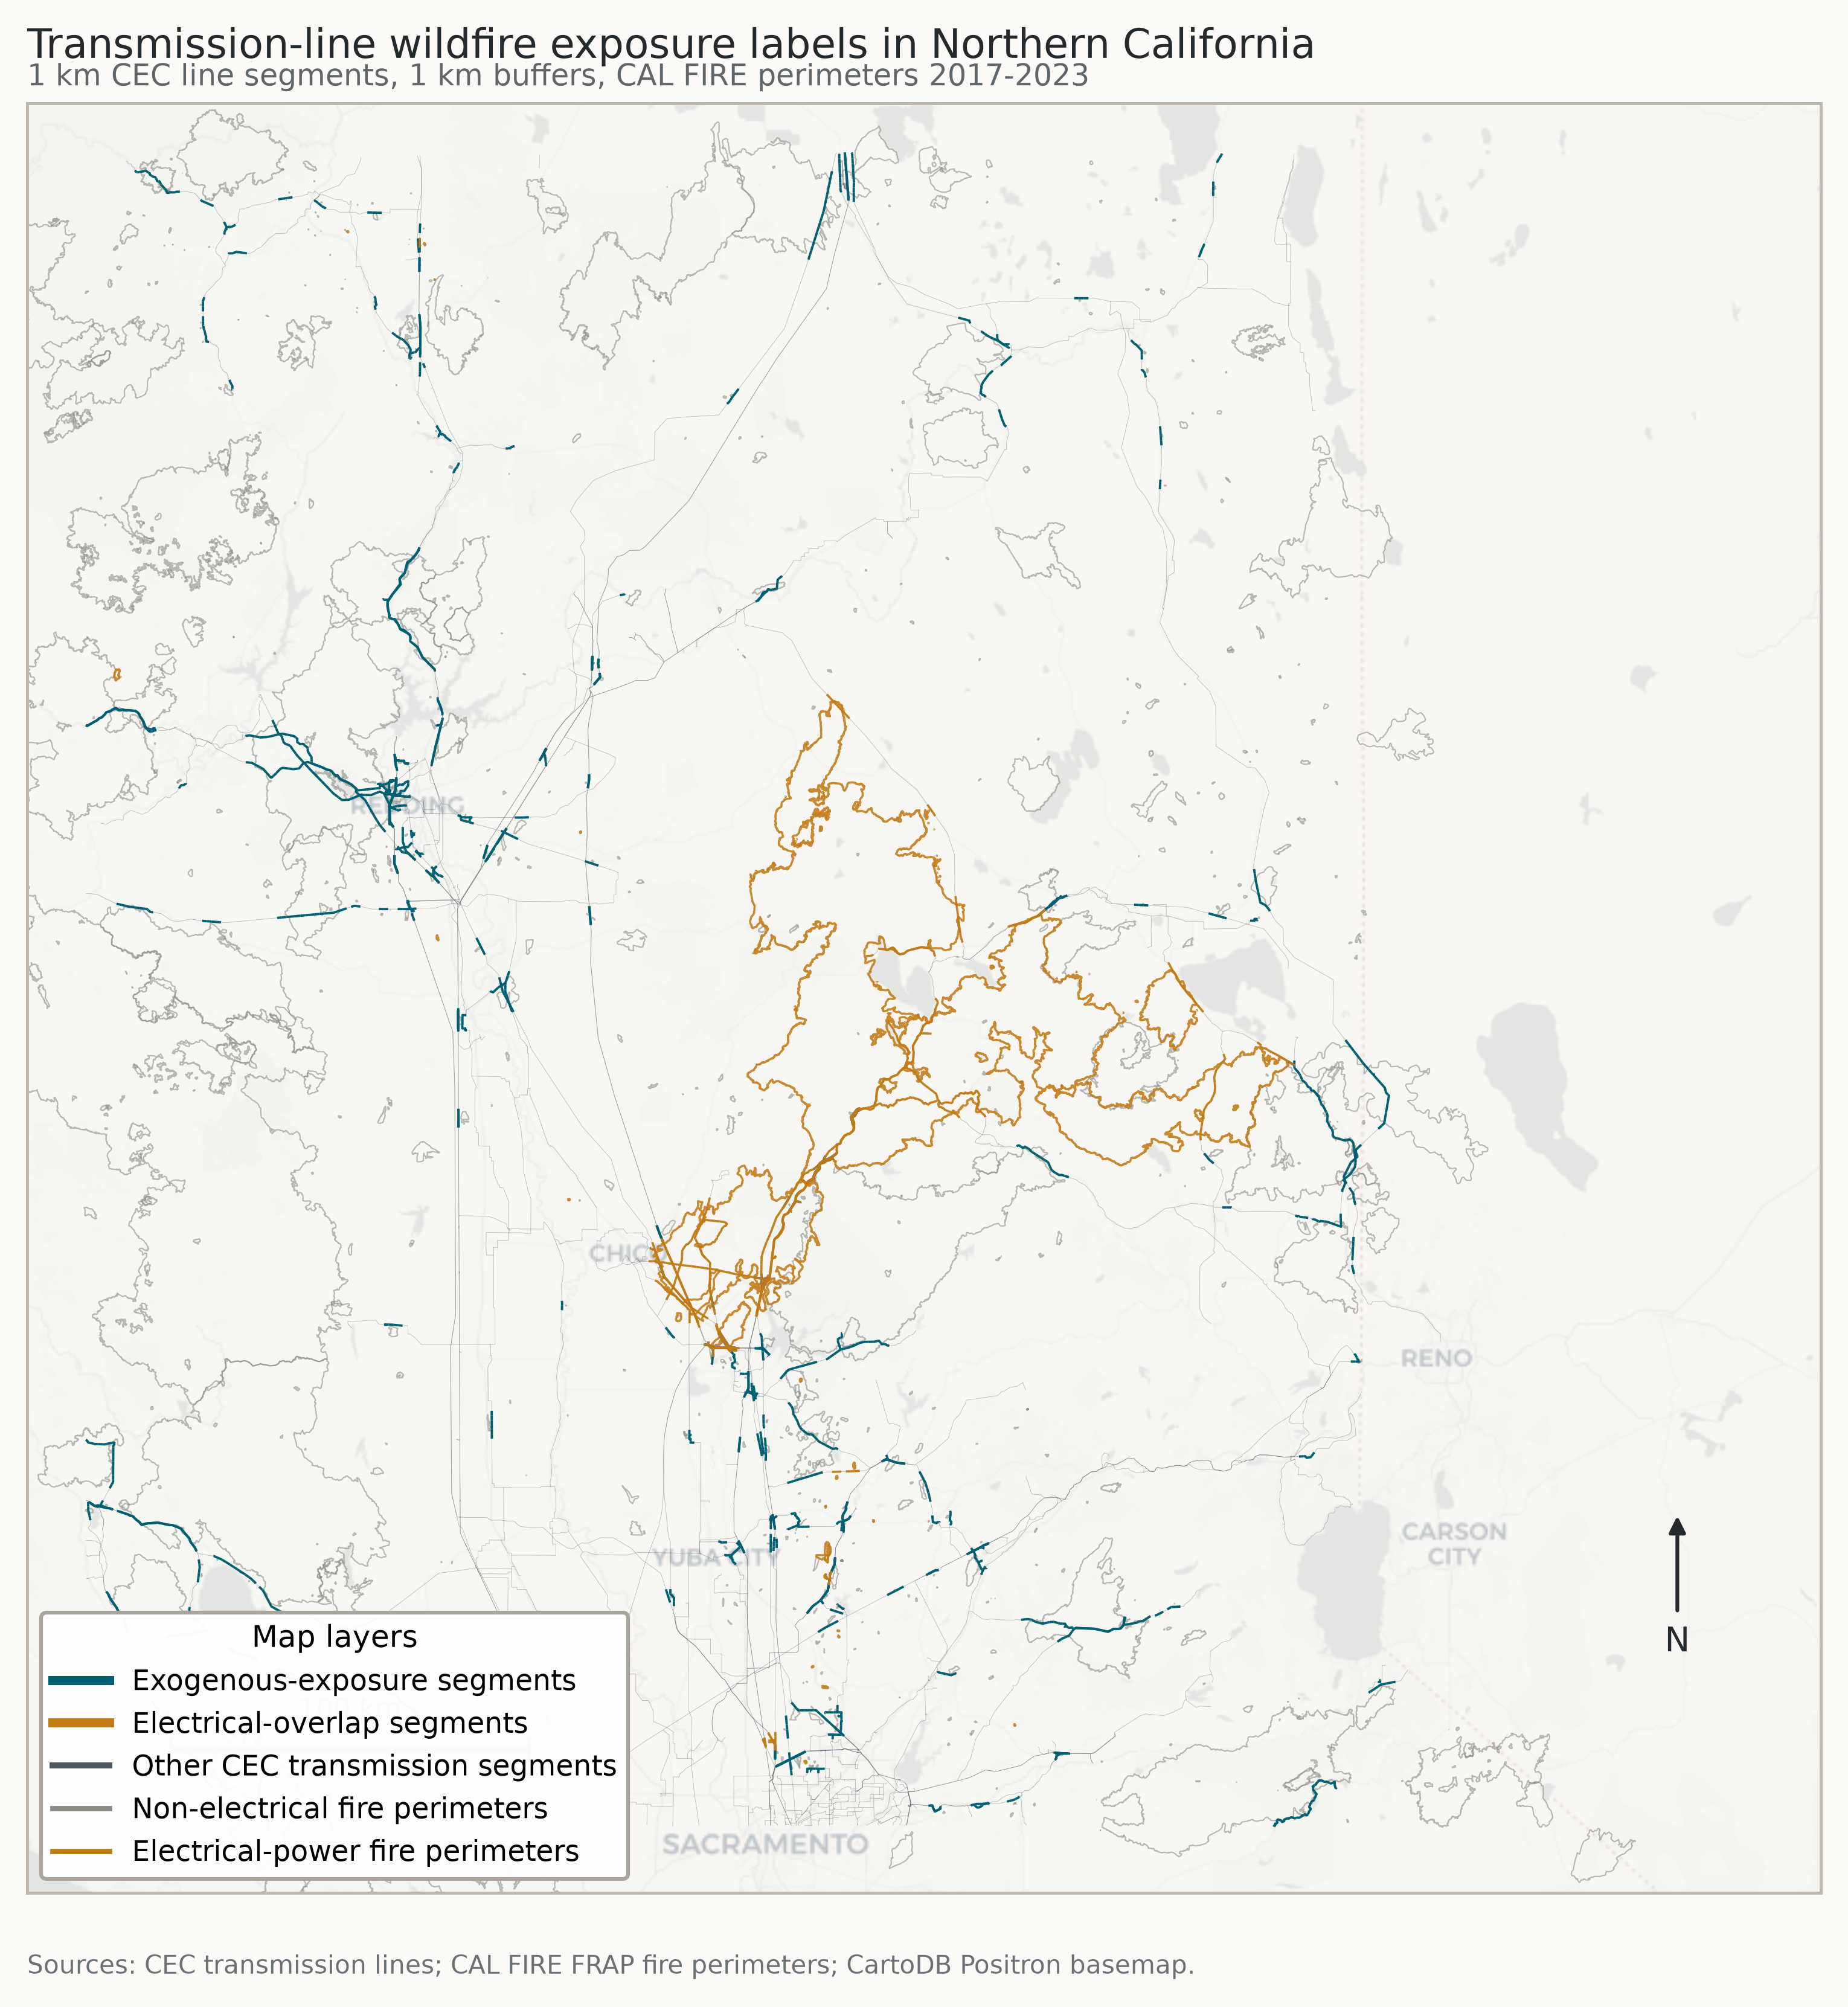
\includegraphics[width=0.94\textwidth]{sci_phase1/fig1_study_area_transmission_fire_labels.png}
  \caption{Study region, public transmission-line segments, and annual exposure labels.}
  \label{fig:study-area}
\end{figure}

\subsection{Public Data Sources}

\autoref{tab:data-sources} summarizes the public data sources. The processed
panel contains 11,255 line segments and 78,785 segment-year observations. CEC
transmission lines provide receptor-asset geometries
\citep{cecTransmissionLines}. CAL FIRE FRAP fire perimeters provide annual
overlap labels \citep{calfireFirePerimeters}. gridMET provides daily
meteorological fields that are summarized annually
\citep{abatzoglou2013gridmet}. LANDFIRE provides static fuel and canopy context
\citep{rollins2009landfire}; this workflow uses LF2024
\citep{landfire2024update}, with product coding and decoded units following
LANDFIRE documentation \citep{landfireDictionary}. Terrain covariates are
derived from USGS 3DEP elevation data \citep{usgs3dep}.

\begin{table}[!htbp]
  \centering
  \footnotesize
  \setlength{\tabcolsep}{3pt}
  \caption{Public data sources and analytical roles.}
  \label{tab:data-sources}
  \begin{tabular}{L{0.16\textwidth} L{0.18\textwidth} L{0.16\textwidth} L{0.14\textwidth} L{0.25\textwidth}}
    \toprule
    Dataset & Source & Resolution / unit & Version or years & Role and caveat \\
    \midrule
    Transmission lines & California Energy Commission & Public line geometry & Current public release & Receptor assets only; not equipment-failure data. \\
    Fire perimeters & CAL FIRE FRAP & Perimeter polygons with cause fields & 2017--2023 subset & Exposure labels; not damage or outage observations. \\
    gridMET & University of Idaho gridMET & Daily weather, annual summaries & 2017--2023 & Observed annual weather covariates. \\
    LANDFIRE & LANDFIRE LF2024 & Fuel and canopy rasters & LF2024 & Static fuel-structure covariates; time-matched sensitivity is needed. \\
    USGS 3DEP & USGS 3DEP & Elevation raster & Current public DEM & Terrain covariate; not a fire-spread model. \\
    \bottomrule
  \end{tabular}
\end{table}

\section{Label Construction}

Let $i$ index line segments, $t$ years, and $j$ individual fire perimeters.
Let $B_i$ be the segment buffer and $P_j$ be fire perimeter $j$. The main
external exposure label is
\begin{equation}
  y^{exo}_{it}
  =
  \ind\left\{
  \exists j:\; \mathrm{year}(j)=t,\;
  B_i \cap P_j \neq \emptyset,\;
  \mathrm{CAUSE}_j \neq 11
  \right\}.
  \label{eq:y-exo}
\end{equation}
CAL FIRE CAUSE = 11 denotes Electrical Power. The exclusion in
\autoref{eq:y-exo} is used to avoid mixing external exposure with
electrical-power fire cause in the main validation target. It does not assert
that remaining fires cannot affect or be affected by transmission assets.

Four annual labels are retained (\autoref{tab:label-algorithm}). The all-fire
label records any perimeter overlap. The exogenous label is the main target.
The strict label further excludes Equipment Use. Electrical-power overlap is a
diagnostic only and is not interpreted as ignition probability.

\begin{table}[!htbp]
  \centering
  \scriptsize
  \setlength{\tabcolsep}{2pt}
  \caption{Annual segment-year labels. Labels are not mutually exclusive because multiple perimeters can overlap a segment-year.}
  \label{tab:label-algorithm}
  \begin{tabular}{L{0.20\textwidth} L{0.42\textwidth} r L{0.22\textwidth}}
    \toprule
    Label & Definition & Positives & Interpretation \\
    \midrule
    All-fire exposure & Any 1 km segment-buffer intersection with a CAL FIRE perimeter & 3,187 & Broad exposure screen. \\
    Exogenous exposure & Any overlap after excluding CAUSE = 11 & 2,331 & Main external exposure target. \\
    Strict exogenous exposure & Excludes CAUSE in \{Electrical Power, Equipment Use\} & 2,075 & Sensitivity label. \\
    Electrical-power overlap & Any overlap with CAUSE = 11 & 885 & Diagnostic only. \\
    Mixed exogenous/electrical rows & Segment-years with both exogenous and electrical-power overlaps & 29 & Multiple-fire overlap diagnostic. \\
    \bottomrule
  \end{tabular}
\end{table}

\begin{figure}[!htbp]
  \centering
  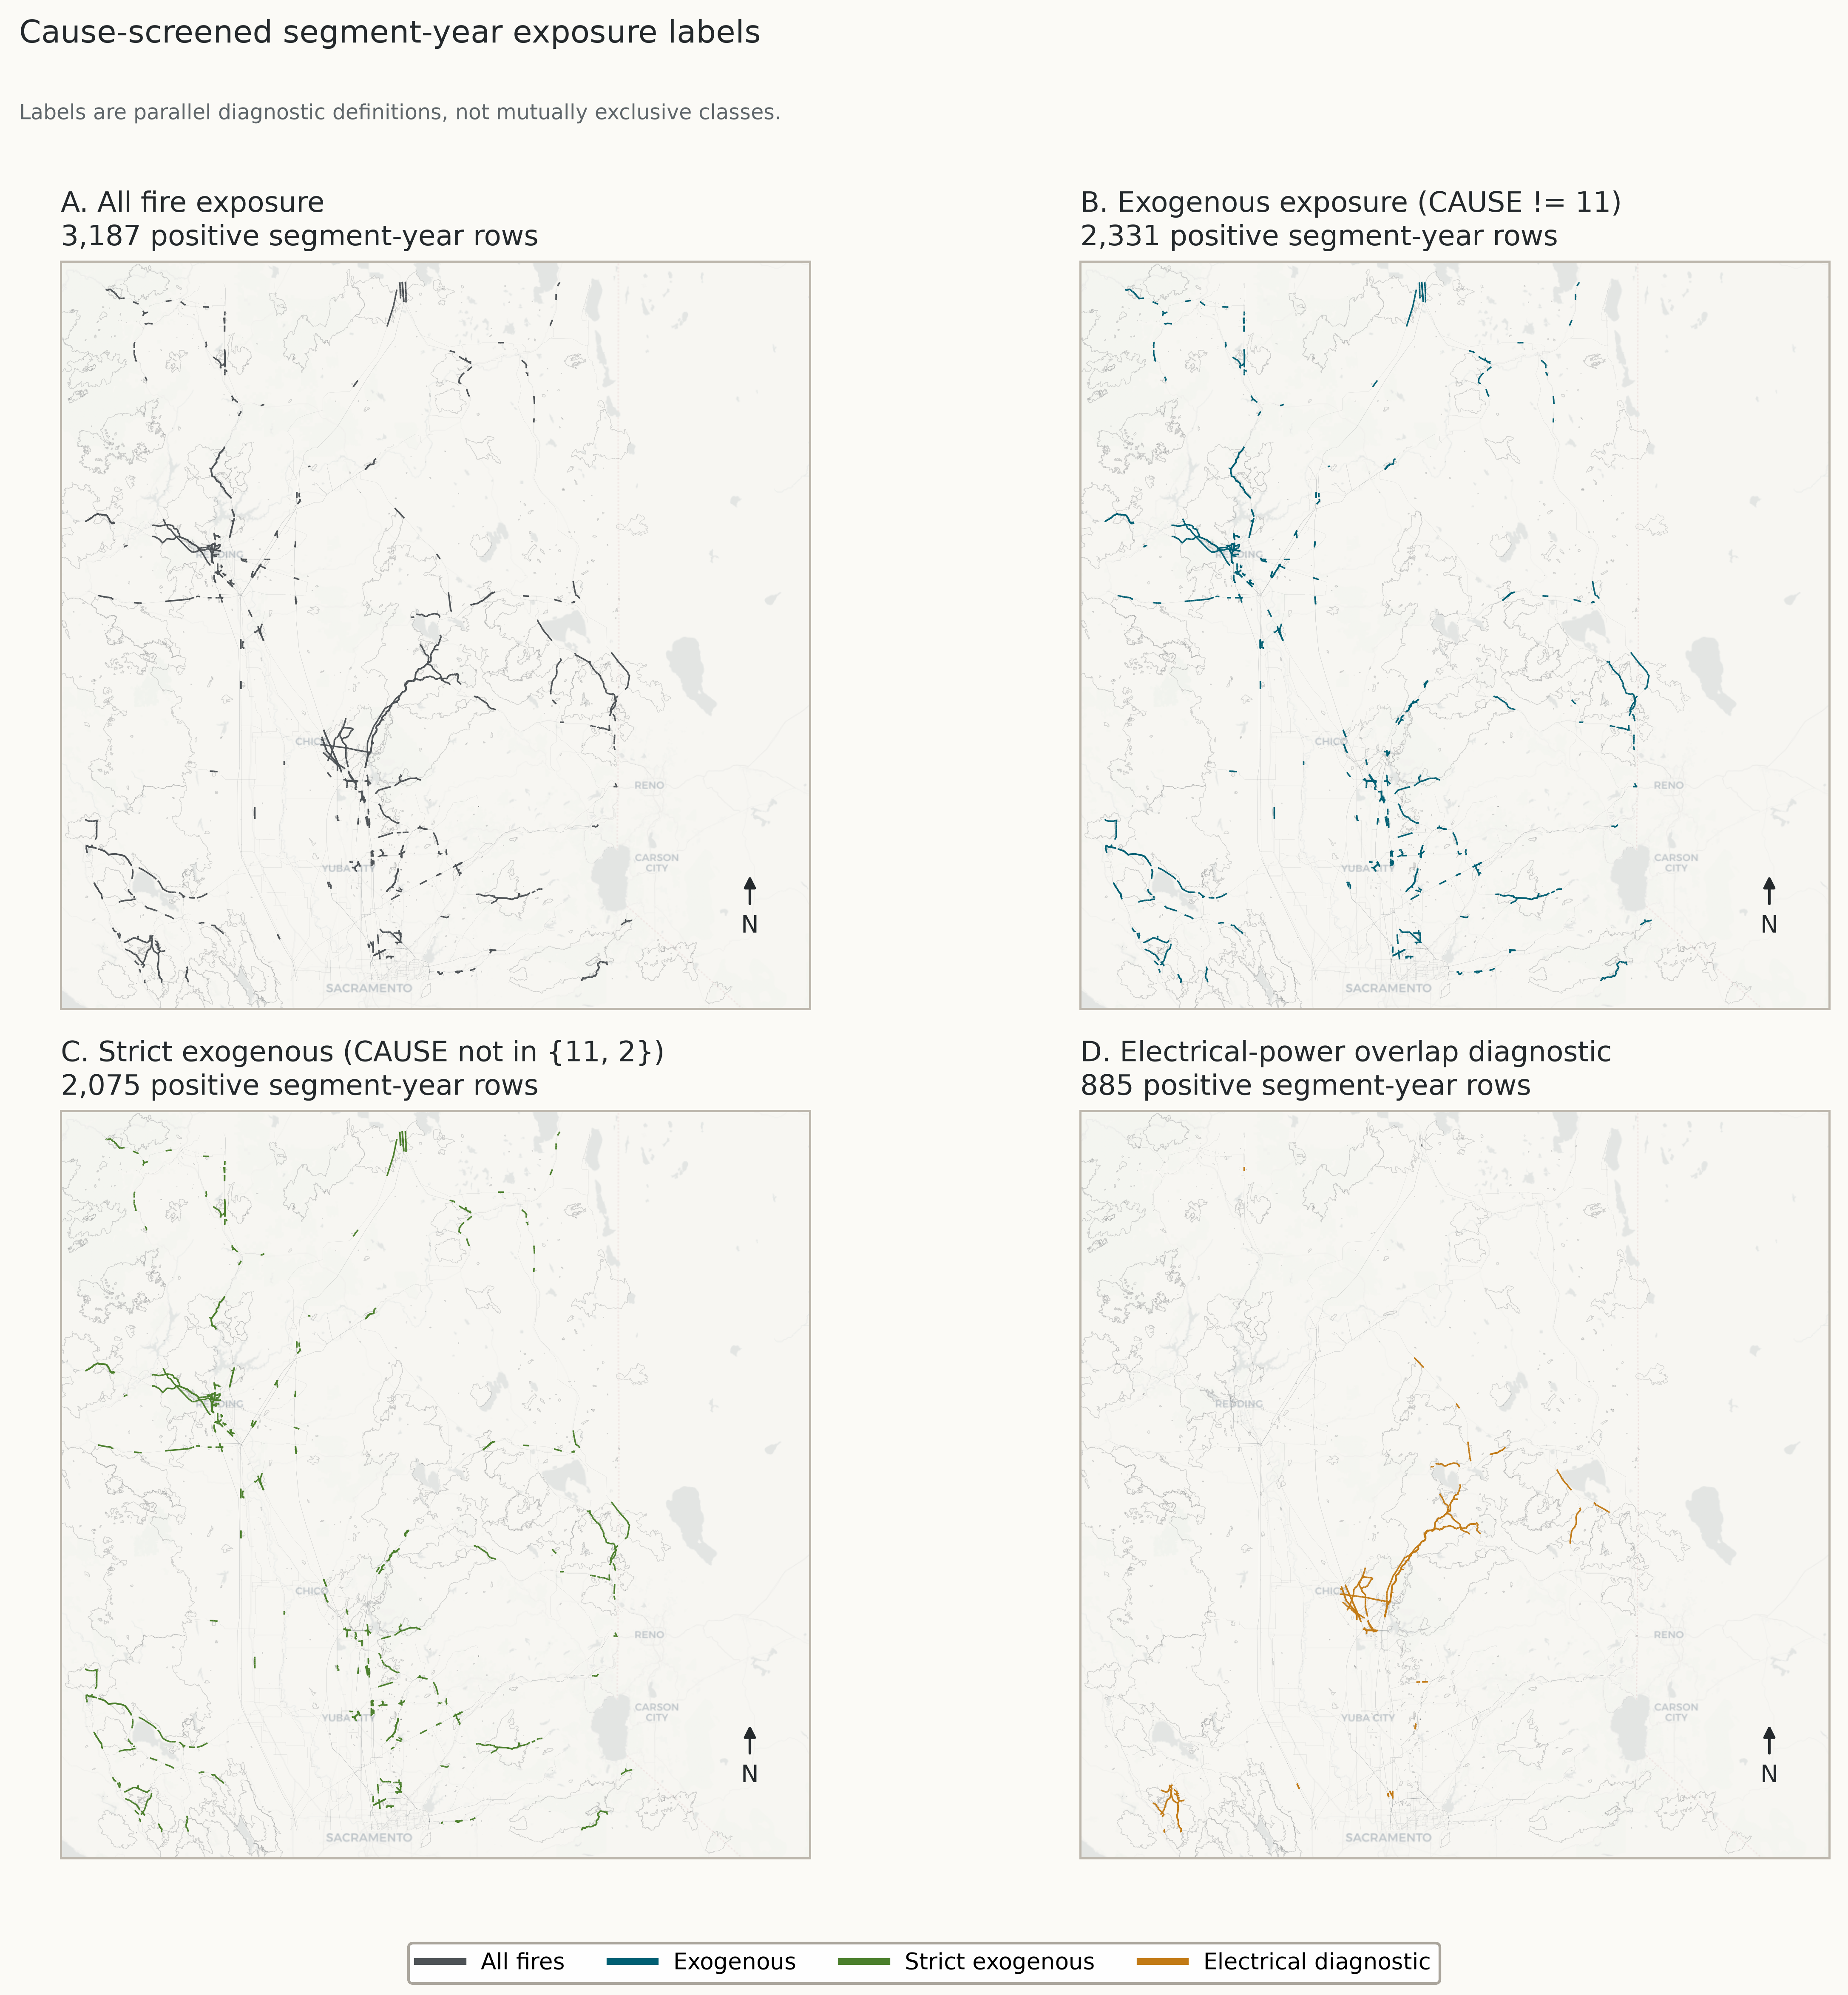
\includegraphics[width=0.94\textwidth]{sci_phase1/fig2_cause_screened_label_maps.png}
  \caption{Cause-screened exposure labels used for receptor-asset validation.}
  \label{fig:cause-screening}
\end{figure}

\begin{figure}[!htbp]
  \centering
  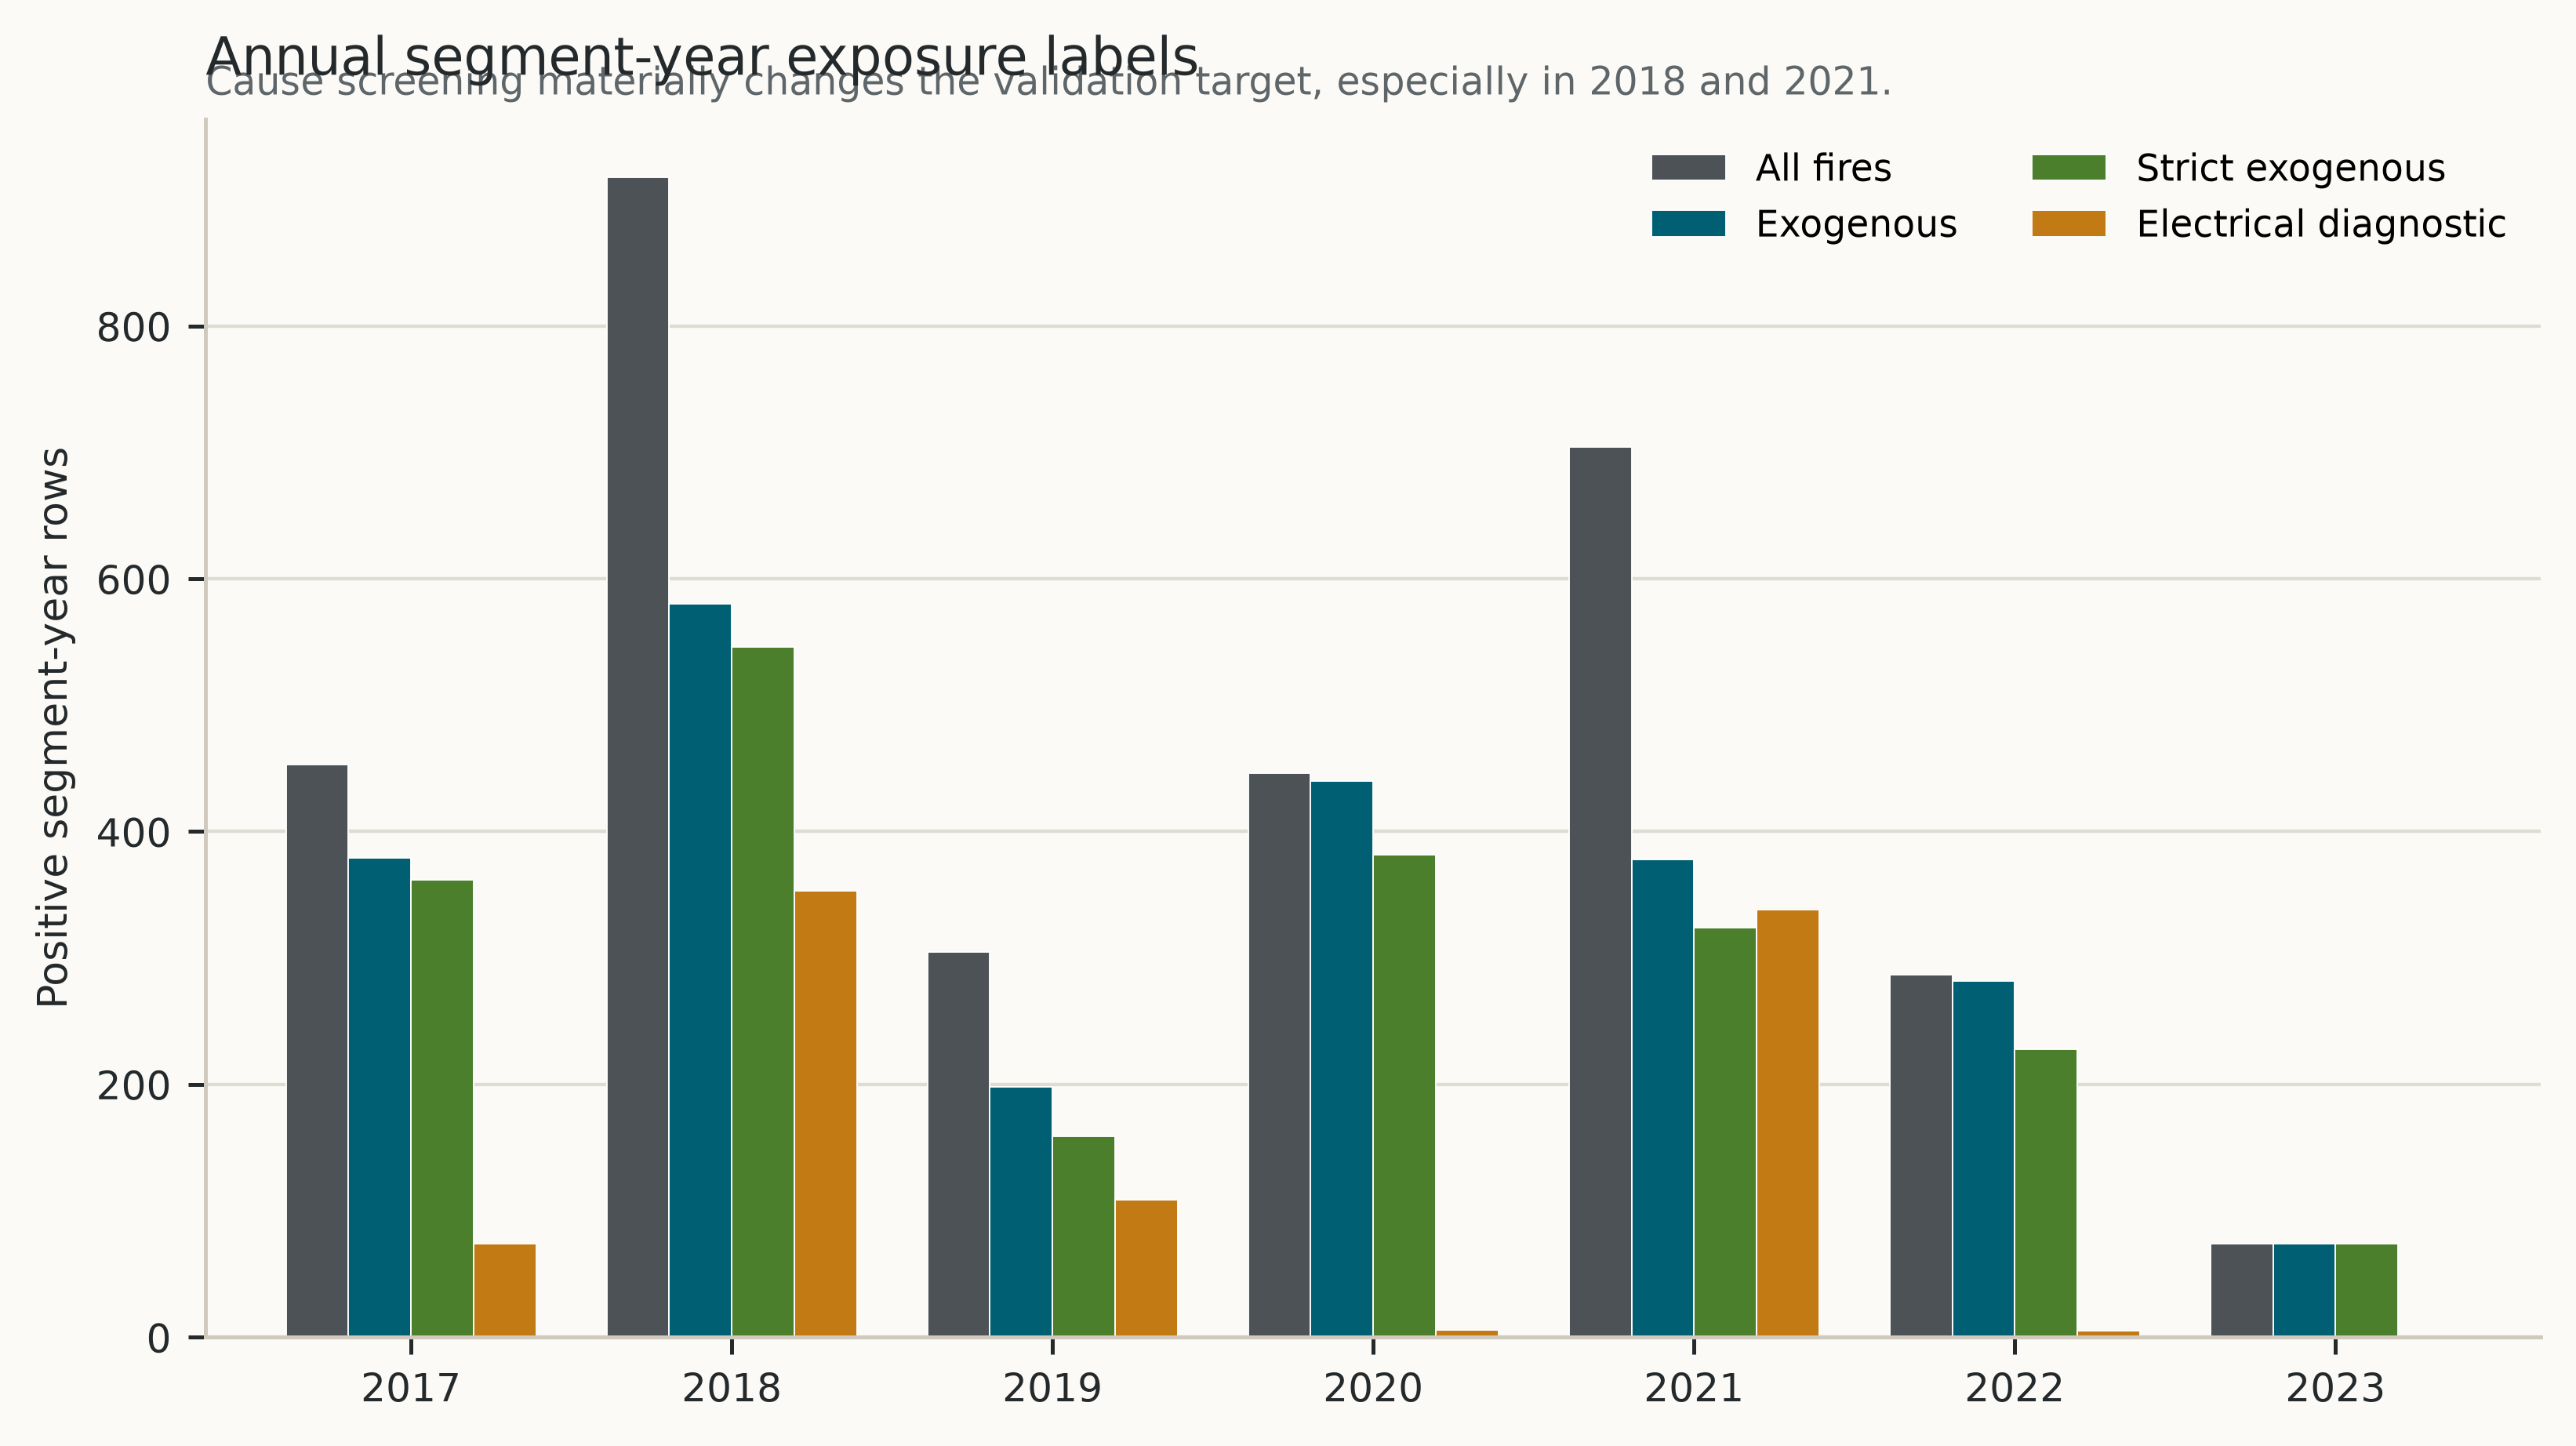
\includegraphics[width=0.88\textwidth]{sci_phase1/fig3_annual_segment_year_label_counts.png}
  \caption{Annual segment-year label counts.}
  \label{fig:annual-labels}
\end{figure}
\FloatBarrier

\section{Methods}

\subsection{Covariate Construction}

The feature core combines observed annual gridMET dryness and wind summaries,
USGS terrain, LANDFIRE canopy/fuel-structure variables, and simple
physics-guided indices. VPD and related fuel-aridity metrics have established
links to western-US fire activity \citep{abatzoglouWilliams2016wildfire}. ERC
and BI are National Fire Danger Rating System quantities
\citep{deeming1977nfdrs}; recent NFDRS modernization has also emphasized
improved live- and dead-fuel-moisture calculations \citep{jolly2024nfdrs}. The
engineered indices below are study-specific standardized composites, not
official NFDRS indices.

\begin{table}[!htbp]
  \centering
  \scriptsize
  \setlength{\tabcolsep}{2pt}
  \caption{Exact construction of model covariates. Spatial extraction follows the processing scripts: gridMET annual aggregates are sampled from the nearest grid cell to the segment midpoint; raster covariates are sampled at the segment midpoint.}
  \label{tab:covariate-construction}
  \begin{tabular}{L{0.14\textwidth} L{0.11\textwidth} L{0.15\textwidth} L{0.17\textwidth} L{0.17\textwidth} L{0.17\textwidth}}
    \toprule
    Variable & Source & Raw unit & Temporal aggregation & Spatial extraction & Role/sign in engineered index \\
    \midrule
    VPD & gridMET & kPa & annual p95 & nearest cell to segment midpoint & dryness, positive \\
    ERC & gridMET & NFDRS index & annual p95 & nearest cell to segment midpoint & dryness, positive \\
    BI & gridMET & NFDRS index & annual p95 & nearest cell to segment midpoint & dryness, positive \\
    wind & gridMET & m s$^{-1}$ & annual p95 & nearest cell to segment midpoint & dryness, positive \\
    FM100 & gridMET & percent & annual p05 & nearest cell to segment midpoint & dryness, negative \\
    FM1000 & gridMET & percent & annual p05 & nearest cell to segment midpoint & dryness, negative \\
    RMIN & gridMET & percent & annual p05 & nearest cell to segment midpoint & dryness, negative \\
    PR & gridMET & mm & annual sum & nearest cell to segment midpoint & dryness, negative \\
    elevation & USGS 3DEP & m & static & raster sample at segment midpoint & deterministic score, positive \\
    canopy cover & LANDFIRE LF2024 & percent & static & raster sample at segment midpoint & fuel index, positive \\
    canopy height & LANDFIRE LF2024 & raw/10 m & static & raster sample at segment midpoint & fuel index, positive \\
    canopy base height & LANDFIRE LF2024 & raw/10 m & static & raster sample at segment midpoint & selected model covariate; not in fuel index \\
    canopy bulk density & LANDFIRE LF2024 & raw/100 kg m$^{-3}$ & static & raster sample at segment midpoint & fuel index, positive \\
    \bottomrule
  \end{tabular}
\end{table}

Let $z(\cdot)$ denote training-period standardization. The dryness index is
\begin{equation}
  \begin{split}
    d_{it}
    &=
    \frac{z(\mathrm{VPD}_{it})+z(\mathrm{ERC}_{it})+z(\mathrm{BI}_{it})+
    z(\mathrm{wind}_{it})}{4}\\
    &\quad -
    \frac{z(\mathrm{FM100}_{it})+z(\mathrm{FM1000}_{it})+
    z(\mathrm{RMIN}_{it})+z(\mathrm{PR}_{it})}{4}.
  \end{split}
\end{equation}
The fuel-structure index is
\begin{equation}
  f_i =
  \frac{
  z(\mathrm{canopy\ cover}_i)+
  z(\mathrm{canopy\ height}_i)+
  z(\mathrm{canopy\ bulk\ density}_i)
  }{3}.
\end{equation}
The selected core contains the raw public covariates, $d_{it}$, $f_i$, and
$d_{it}f_i$. Canopy base height is included as an additional selected model
covariate but is not part of the fuel-structure index in this specification.
Because $d_{it}$ and $f_i$ are linear composites of raw standardized covariates,
individual coefficients are not interpreted; the physics-guided nonlinear
information enters through the interaction $d_{it}f_i$. LANDFIRE FBFM40 is
categorical and is not used in the selected Bayesian or L2 logistic core.

\subsection{Deterministic Comparator}

The deterministic comparator is a transparent, calibrated physics-guided score:
\begin{equation}
  r^{det}_{it}
  =
  0.56 d_{it} + 0.30 f_i + 0.14 z(\mathrm{elevation}_i).
\end{equation}
The weights were fixed as an a priori transparent heuristic comparator and were
not optimized on the 2022--2023 holdout. The raw score is clipped to the
training-period 1st--99th percentile range and scaled to $[0,1]$:
\begin{equation}
  s^{det}_{it}
  =
  \frac{
  \operatorname{clip}\left(r^{det}_{it},q^{train}_{0.01},q^{train}_{0.99}\right)
  - q^{train}_{0.01}
  }{
  q^{train}_{0.99}-q^{train}_{0.01}
  }.
\end{equation}
It is then
calibrated with a regularized logistic model,
\begin{equation}
  p^{det}_{it} = \logit^{-1}(\gamma_0+\gamma_1 s^{det}_{it}).
\end{equation}
This gives a single score and calibrated point probability but no posterior
distribution over ranks.

\subsection{Bayesian and L2 Logistic Models}

The Bayesian exposure model is a weakly regularized logistic regression:
\begin{align}
  y^{exo}_{it} &\sim \mathrm{Bernoulli}(p_{it}), \\
  p_{it} &= \logit^{-1}(\alpha+\mathbf{x}_{it}^{\top}\boldsymbol{\beta}),\\
  \alpha &\sim \mathcal{N}(0,5^2), \qquad
  \beta_k \sim \mathcal{N}(0,2^2).
\end{align}
The exact design vector is
\begin{equation}
\begin{split}
\mathbf{x}_{it} =
[
&z(\mathrm{VPD}), z(\mathrm{ERC}), z(\mathrm{BI}), z(\mathrm{wind}),\\
&z(\mathrm{FM100}), z(\mathrm{FM1000}), z(\mathrm{RMIN}), z(\mathrm{PR}),\\
&z(\mathrm{elevation}), z(\mathrm{canopy\ cover}), z(\mathrm{canopy\ height}),\\
&z(\mathrm{canopy\ base\ height}), z(\mathrm{canopy\ bulk\ density}),
d_{it}, f_i, d_{it}f_i
]^\top .
\end{split}
\label{eq:x-vector}
\end{equation}
All entries are centered and scaled using the 2017--2021 training rows before
model fitting.
Weakly informative regularization is commonly used to stabilize logistic
regression coefficients \citep{gelman2008weakPriors}. The posterior is
approximated by a Laplace approximation around the posterior mode
$\hat{\theta}$,
\begin{equation}
  p(\theta \mid \mathcal{D}) \approx
  \mathcal{N}\left(\hat{\theta},\; H(\hat{\theta})^{-1}\right),
\end{equation}
where $H(\hat{\theta})$ is the negative Hessian of the log posterior
\citep{tierneyKadane1986laplace}. A Gaussian prior on coefficients is
equivalent to an L2 penalty at the posterior mode; similar discrimination
between Bayesian Laplace and L2 logistic is therefore expected. The Bayesian
layer is retained because posterior draws support rank and threshold decision
quantities.

For posterior draw $s$, segment exposure over holdout years $T^\star$ is
\begin{equation}
  \bar{p}_{i}^{(s)}
  =
  \frac{1}{|T^\star|}
  \sum_{t\in T^\star} \logit^{-1}
  \left(\alpha^{(s)}+\mathbf{x}_{it}^{\top}\boldsymbol{\beta}^{(s)}\right).
\end{equation}
The decision quantities are
\begin{align}
  q_i
  &= P(\bar{p}_i > \tau \mid \mathcal{D})
  \approx
  \frac{1}{S}\sum_{s=1}^{S}
  \ind\{\bar{p}_{i}^{(s)}>\tau\},\\
  \rho_i
  &= P(\mathrm{rank}_{\downarrow}(\bar{p}_i) \le K \mid \mathcal{D})
  \approx
  \frac{1}{S}\sum_{s=1}^{S}
  \ind\{\mathrm{rank}_{\downarrow}(\bar{p}_{i}^{(s)})\le K\}.
\end{align}
Here $\tau=\pi_{train}$ is the training-period prevalence, $K=\lceil0.1N\rceil$,
and $\mathrm{rank}_{\downarrow}$ denotes descending exposure rank.

\begin{figure}[!htbp]
  \centering
  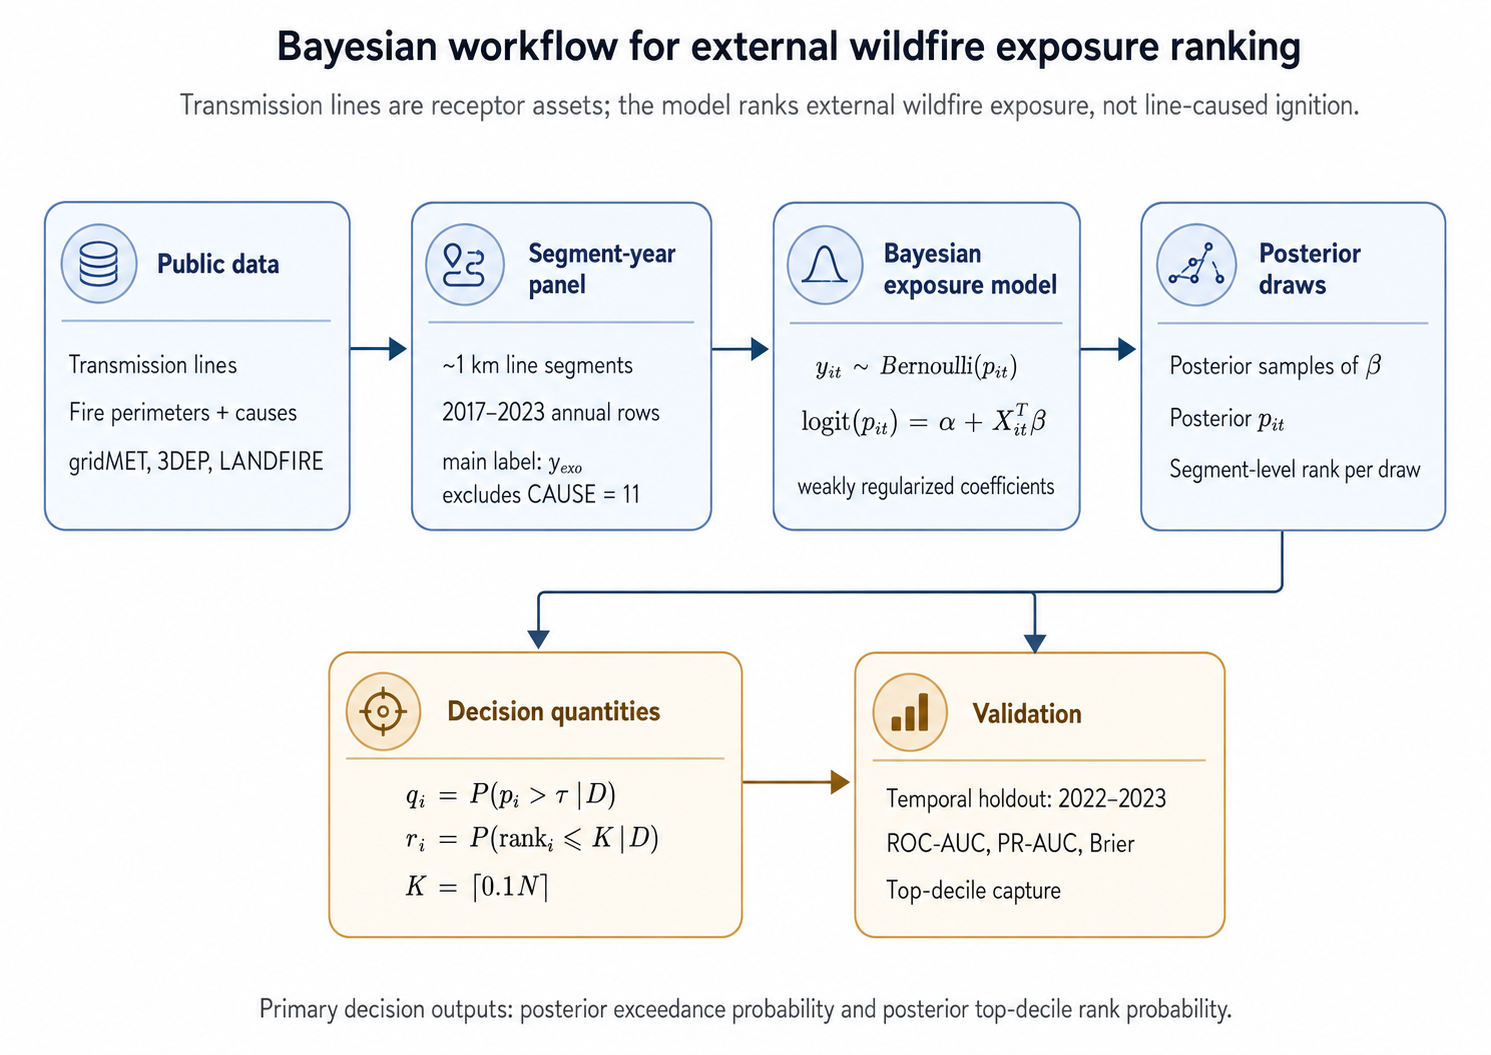
\includegraphics[width=0.92\textwidth]{phase8/phase8_bayesian_method_schematic-2.png}
  \caption{Bayesian workflow for posterior exposure probability and posterior top-decile rank probability.}
  \label{fig:method-schematic}
\end{figure}

\subsection{Baseline Models and Implementation}

All non-Bayesian baselines are fitted with fixed scikit-learn specifications
using the same selected physics core. No hyperparameter is selected using the
2022--2023 comparison. \autoref{tab:baseline-implementation} records the
implementation details needed to reproduce the reported baselines.

\begin{table}[!htbp]
  \centering
  \scriptsize
  \setlength{\tabcolsep}{2pt}
  \caption{Baseline model implementations.}
  \label{tab:baseline-implementation}
  \begin{tabular}{L{0.18\textwidth} L{0.24\textwidth} L{0.20\textwidth} L{0.26\textwidth}}
    \toprule
    Model & Implementation & Class handling & Key fixed parameters \\
    \midrule
    Logistic L2 & StandardScaler + sklearn LogisticRegression & Default class weights & solver = lbfgs; C = 1; max\_iter = 2000; seed = 20260701 \\
    Balanced random forest & sklearn RandomForestClassifier & class\_weight = balanced\_subsample & n\_estimators = 450; min\_samples\_leaf = 12; n\_jobs = -1; seed = 20260701 \\
    Balanced extra trees & sklearn ExtraTreesClassifier & class\_weight = balanced & n\_estimators = 450; min\_samples\_leaf = 12; n\_jobs = -1; seed = 20260701 \\
    Histogram gradient boosting & sklearn HistGradientBoostingClassifier & No explicit class weighting & max\_iter = 260; learning\_rate = 0.035; max\_leaf\_nodes = 24; l2\_regularization = 0.05; seed = 20260701 \\
    \bottomrule
  \end{tabular}
\end{table}

\subsection{Validation Design}

Models are trained on 2017--2021 and evaluated on 2022--2023. The holdout set
contains 22,510 segment-year rows and 356 exogenous exposure positives, giving
a holdout prevalence of 1.5815\%. Precision-recall performance is emphasized
alongside ROC-AUC because PR curves are more informative under heavy class
imbalance \citep{saitoRehmsmeier2015pr}. Probabilistic accuracy is summarized
with the Brier score \citep{brier1950verification}. Brier skill is reported
against the out-of-sample constant probability defined by the training
prevalence, while the holdout-prevalence constant is reported only as a
hindsight reference.

As a preliminary uncertainty check on metric differences, we also compute
$B=120$ paired segment-cluster bootstrap replicates. Each replicate resamples
segment IDs with replacement, retains all holdout-year rows for selected
segments, and recomputes paired PR-AUC and Capture@10 differences. Intervals
are 2.5th--97.5th bootstrap percentiles. This check is not a replacement for
spatial block validation.

\section{Results}

\subsection{Temporal Holdout Performance}

\autoref{tab:main-comparison} summarizes temporal-holdout performance. Bayesian
Laplace and L2 logistic have similar discrimination. In this split, their
top-ranked tails capture more holdout positives than the deterministic
comparator, while the Bayesian point prediction is not materially better than
L2 logistic. The Bayesian contribution is therefore interpreted as a posterior
decision layer rather than as broad classification superiority. An initial Stan
run reproduced the Laplace point-ranking metrics; full convergence summaries
and posterior predictive diagnostics remain future work.

\begin{table}[!htbp]
  \centering
  \small
  \caption{Temporal-holdout comparison for 2022--2023 exogenous exposure.}
  \label{tab:main-comparison}
  \begin{tabular}{lrrrrr}
    \toprule
    Model & ROC-AUC & PR-AUC & Brier & Row top 10\% & Segment top 10\% \\
    \midrule
    ML logistic L2 & 0.663 & 0.039 & 0.015713 & 0.289 & 0.216 \\
    Bayesian Laplace & 0.662 & 0.038 & 0.015718 & 0.289 & 0.216 \\
    Deterministic calibrated & 0.651 & 0.028 & 0.015734 & 0.219 & 0.118 \\
    Balanced extra trees & 0.617 & 0.022 & 0.056091 & 0.180 & 0.104 \\
    Histogram gradient boosting & 0.553 & 0.019 & 0.016647 & 0.132 & 0.149 \\
    Balanced random forest & 0.568 & 0.018 & 0.034539 & 0.107 & 0.152 \\
    \bottomrule
  \end{tabular}
\end{table}

\begin{figure}[!htbp]
  \centering
  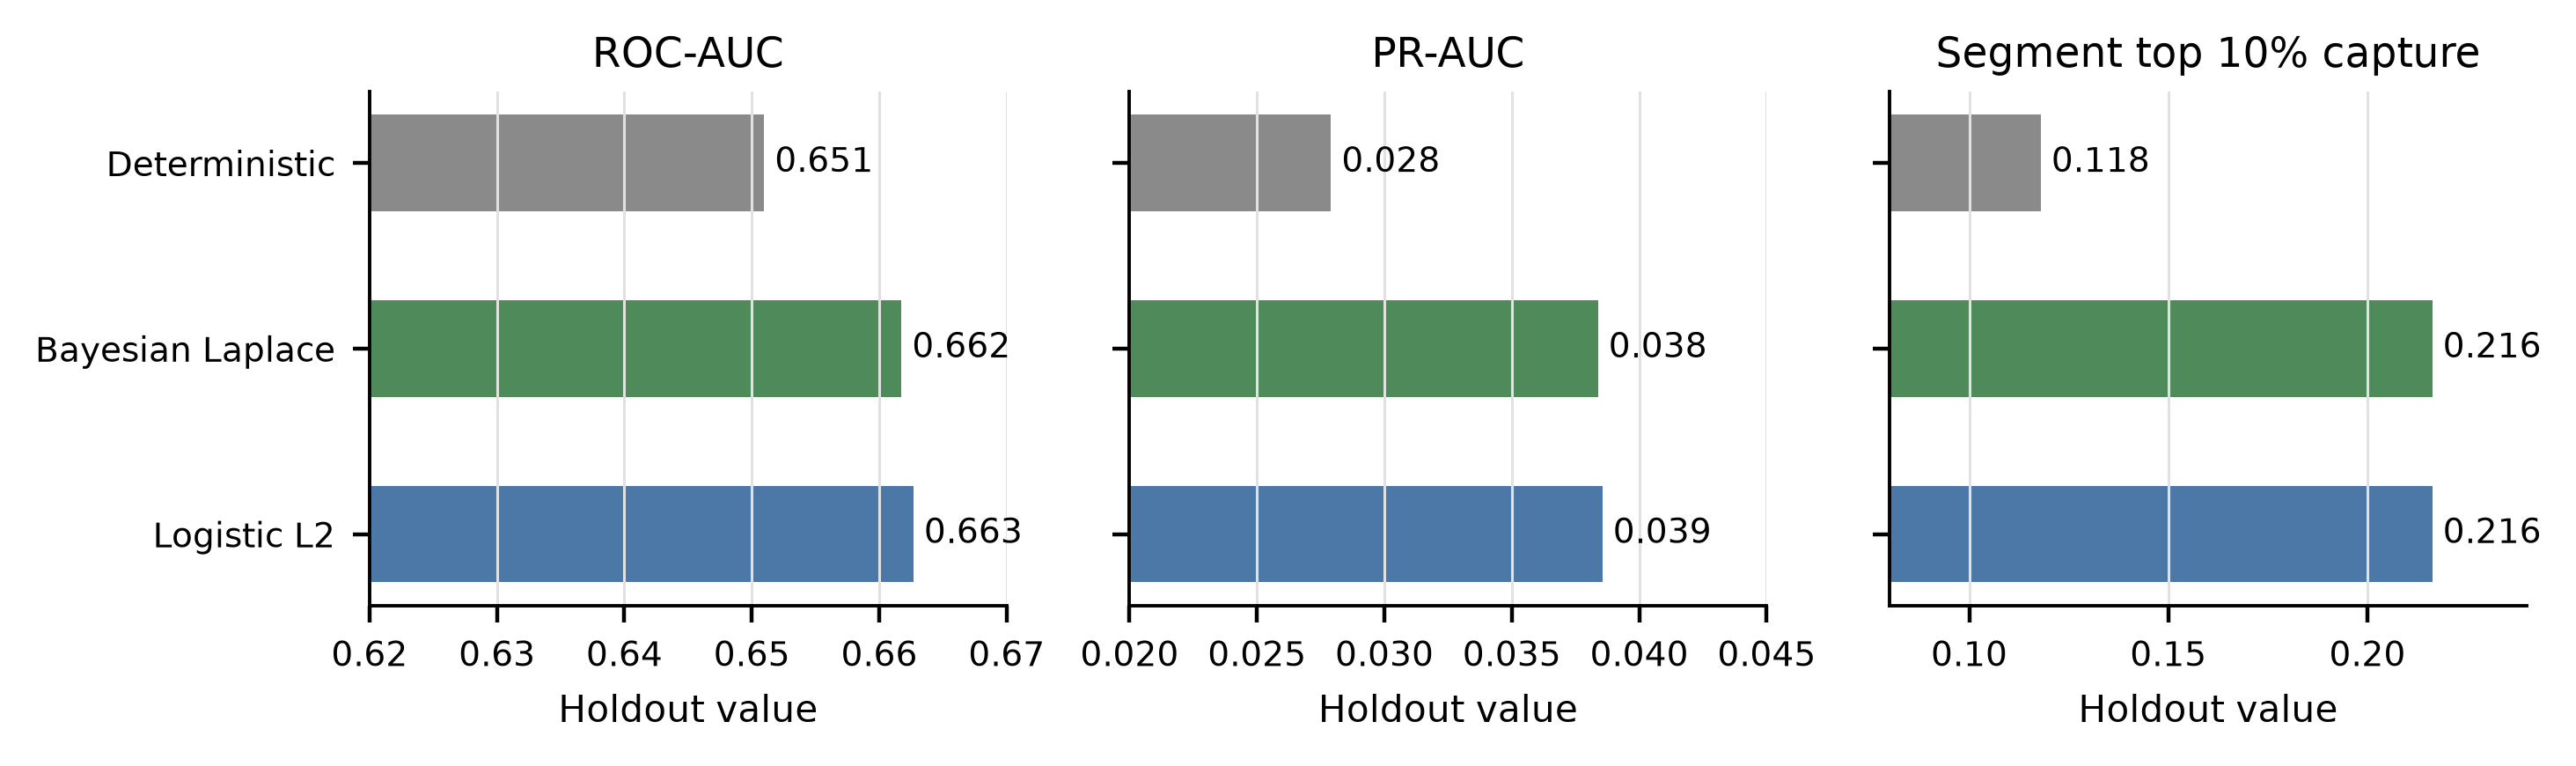
\includegraphics[width=0.94\textwidth]{sci_minorrev_20260708/fig_holdout_metrics.png}
  \caption{Key 2022--2023 temporal-holdout metrics for the deterministic comparator, Bayesian Laplace posterior mean, and L2 logistic baseline.}
  \label{fig:holdout-metrics}
\end{figure}

\begin{figure}[!htbp]
  \centering
  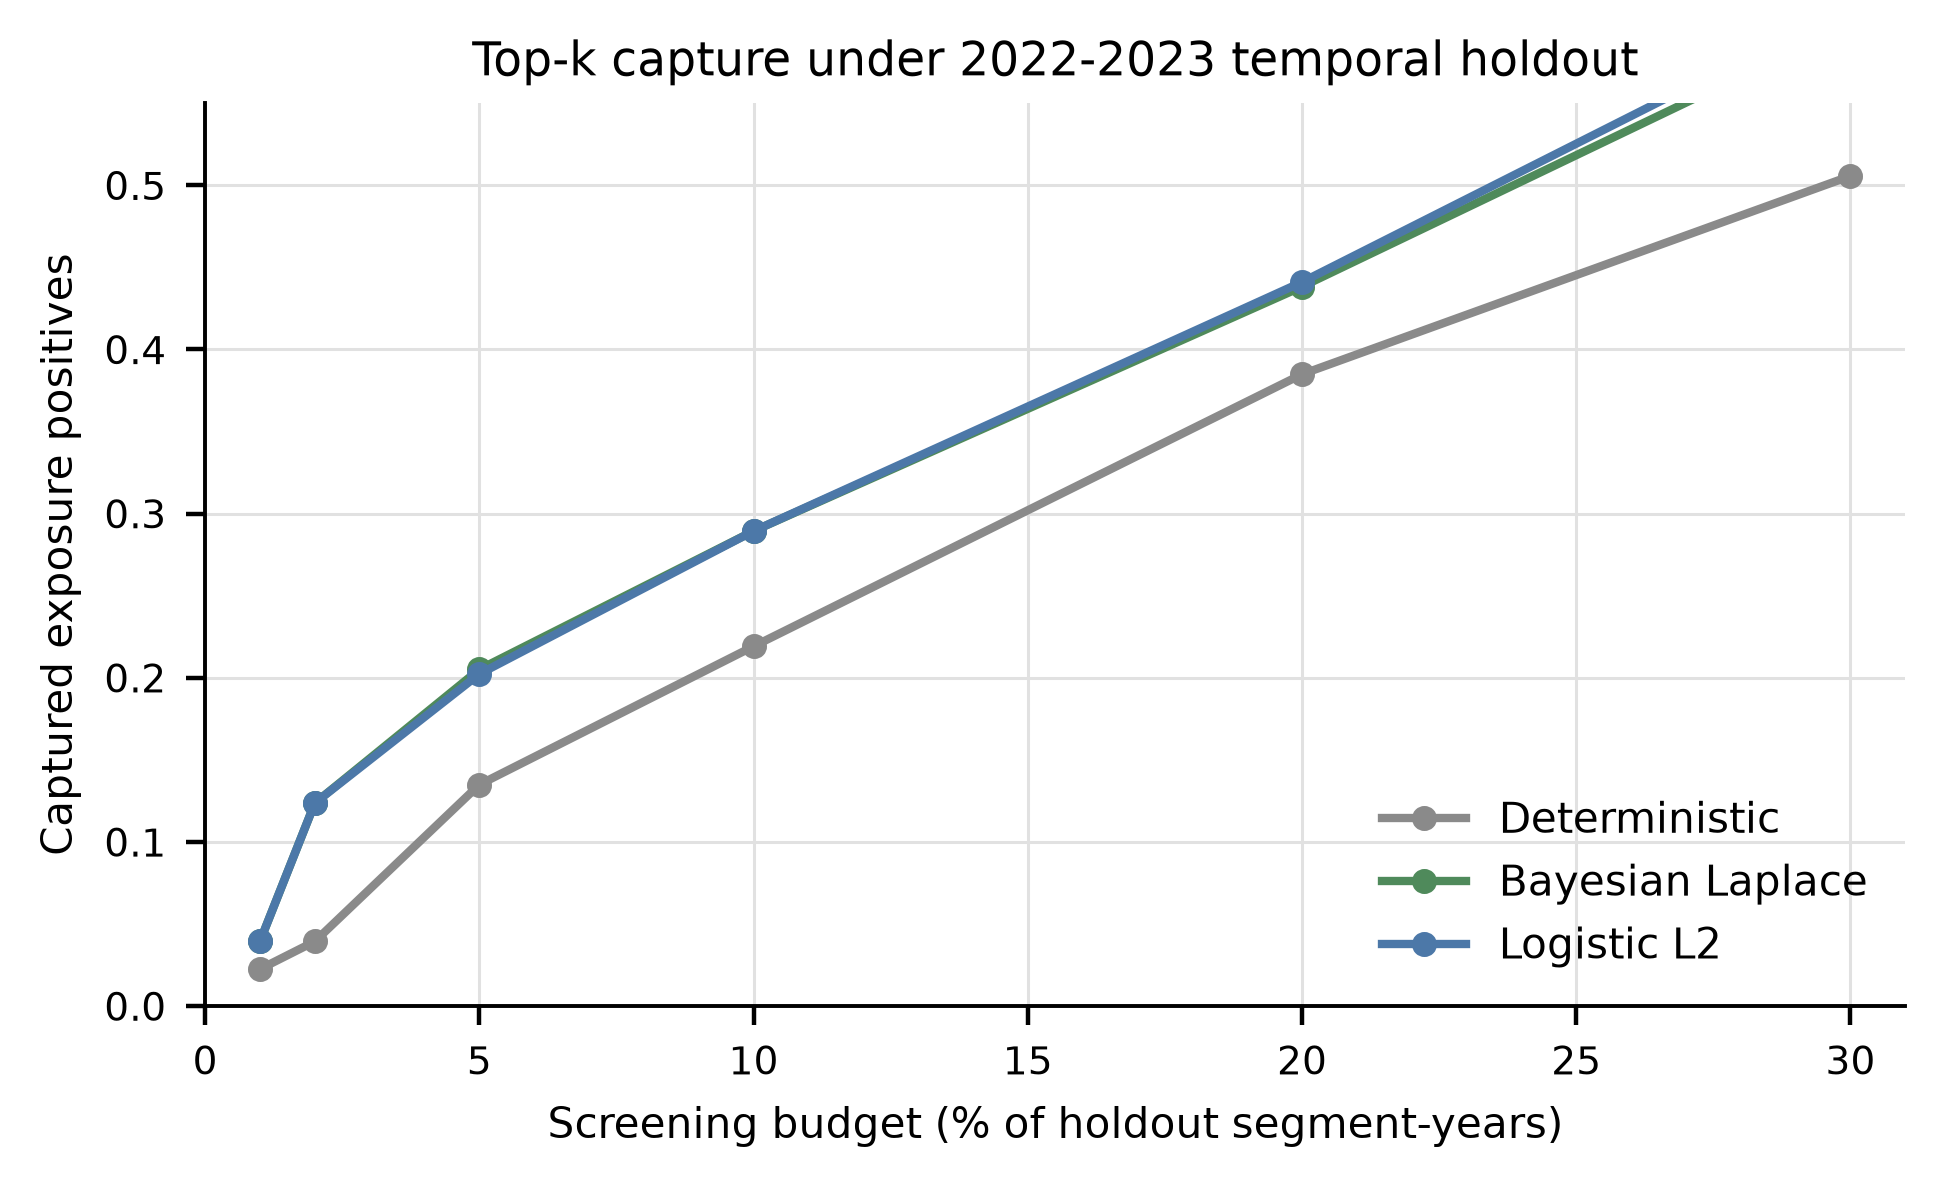
\includegraphics[width=0.82\textwidth]{sci_minorrev_20260708/fig_topk_capture.png}
  \caption{Top-k capture curve under the 2022--2023 temporal holdout. Bayesian Laplace and L2 logistic rankings are close; both select more observed exposure positives than the deterministic comparator in the top-ranked tail of this split.}
  \label{fig:topk-capture}
\end{figure}

\begin{figure}[!htbp]
  \centering
  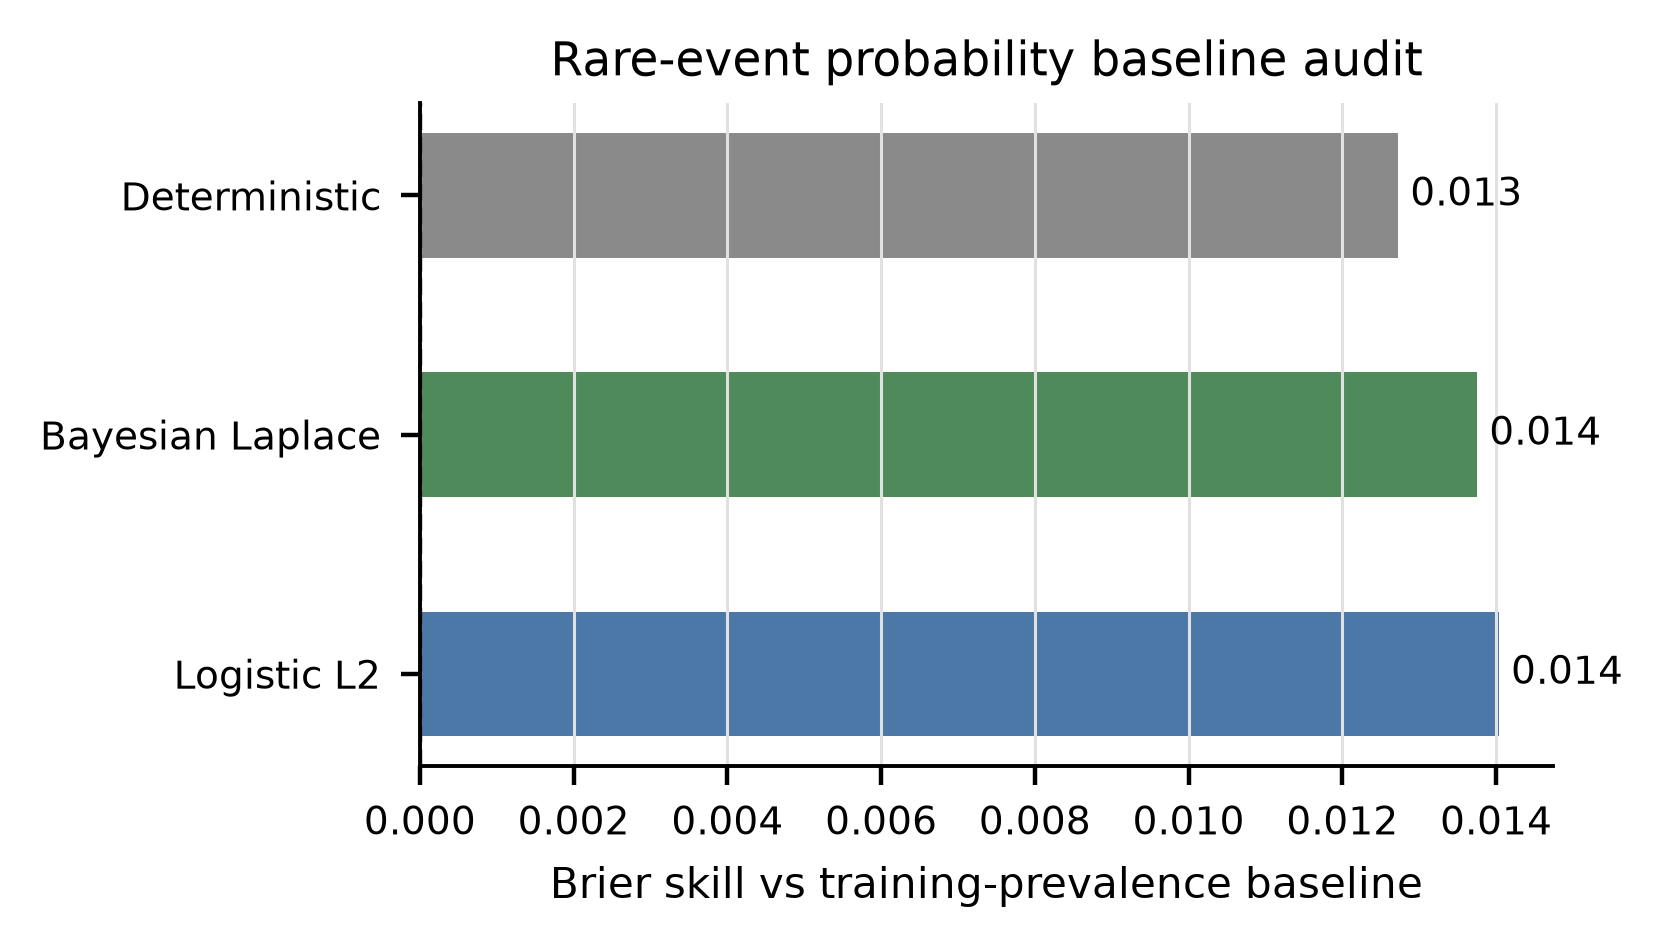
\includegraphics[width=0.70\textwidth]{sci_minorrev_20260708/fig_brier_skill.png}
  \caption{Brier skill relative to the training-prevalence constant probability baseline.}
  \label{fig:brier-skill}
\end{figure}

\begin{table}[!htbp]
  \centering
  \small
  \caption{Rare-event probability baseline audit. Training prevalence is 1,975 / 56,275 = 3.5096\%, giving a training-prevalence constant Brier score of 0.015937 on the holdout. The holdout-prevalence constant reference is 0.015565 and is available only in hindsight.}
  \label{tab:brier-skill}
  \begin{tabular}{lrrrr}
    \toprule
    Model & PR-AUC & PR-AUC / $\pi_{test}$ & Brier & BSS vs $\pi_{train}$ \\
    \midrule
    Logistic L2 & 0.03855 & 2.438 & 0.015713 & 0.0140 \\
    Bayesian Laplace & 0.03838 & 2.427 & 0.015718 & 0.0138 \\
    Deterministic calibrated & 0.02790 & 1.764 & 0.015734 & 0.0127 \\
    \bottomrule
  \end{tabular}
\end{table}

\subsection{Posterior Decision Maps and Method Diagnostics}

The posterior map output should be read as an uncertainty-aware exposure-ranking
diagnostic. In particular, $\rho_i=P(\mathrm{rank}_{\downarrow}\le K\mid
\mathcal{D})$ identifies segments that repeatedly fall into the top decile
under posterior draws. \autoref{fig:posterior-maps} shows the posterior
decision metrics.

\begin{figure}[!htbp]
  \centering
  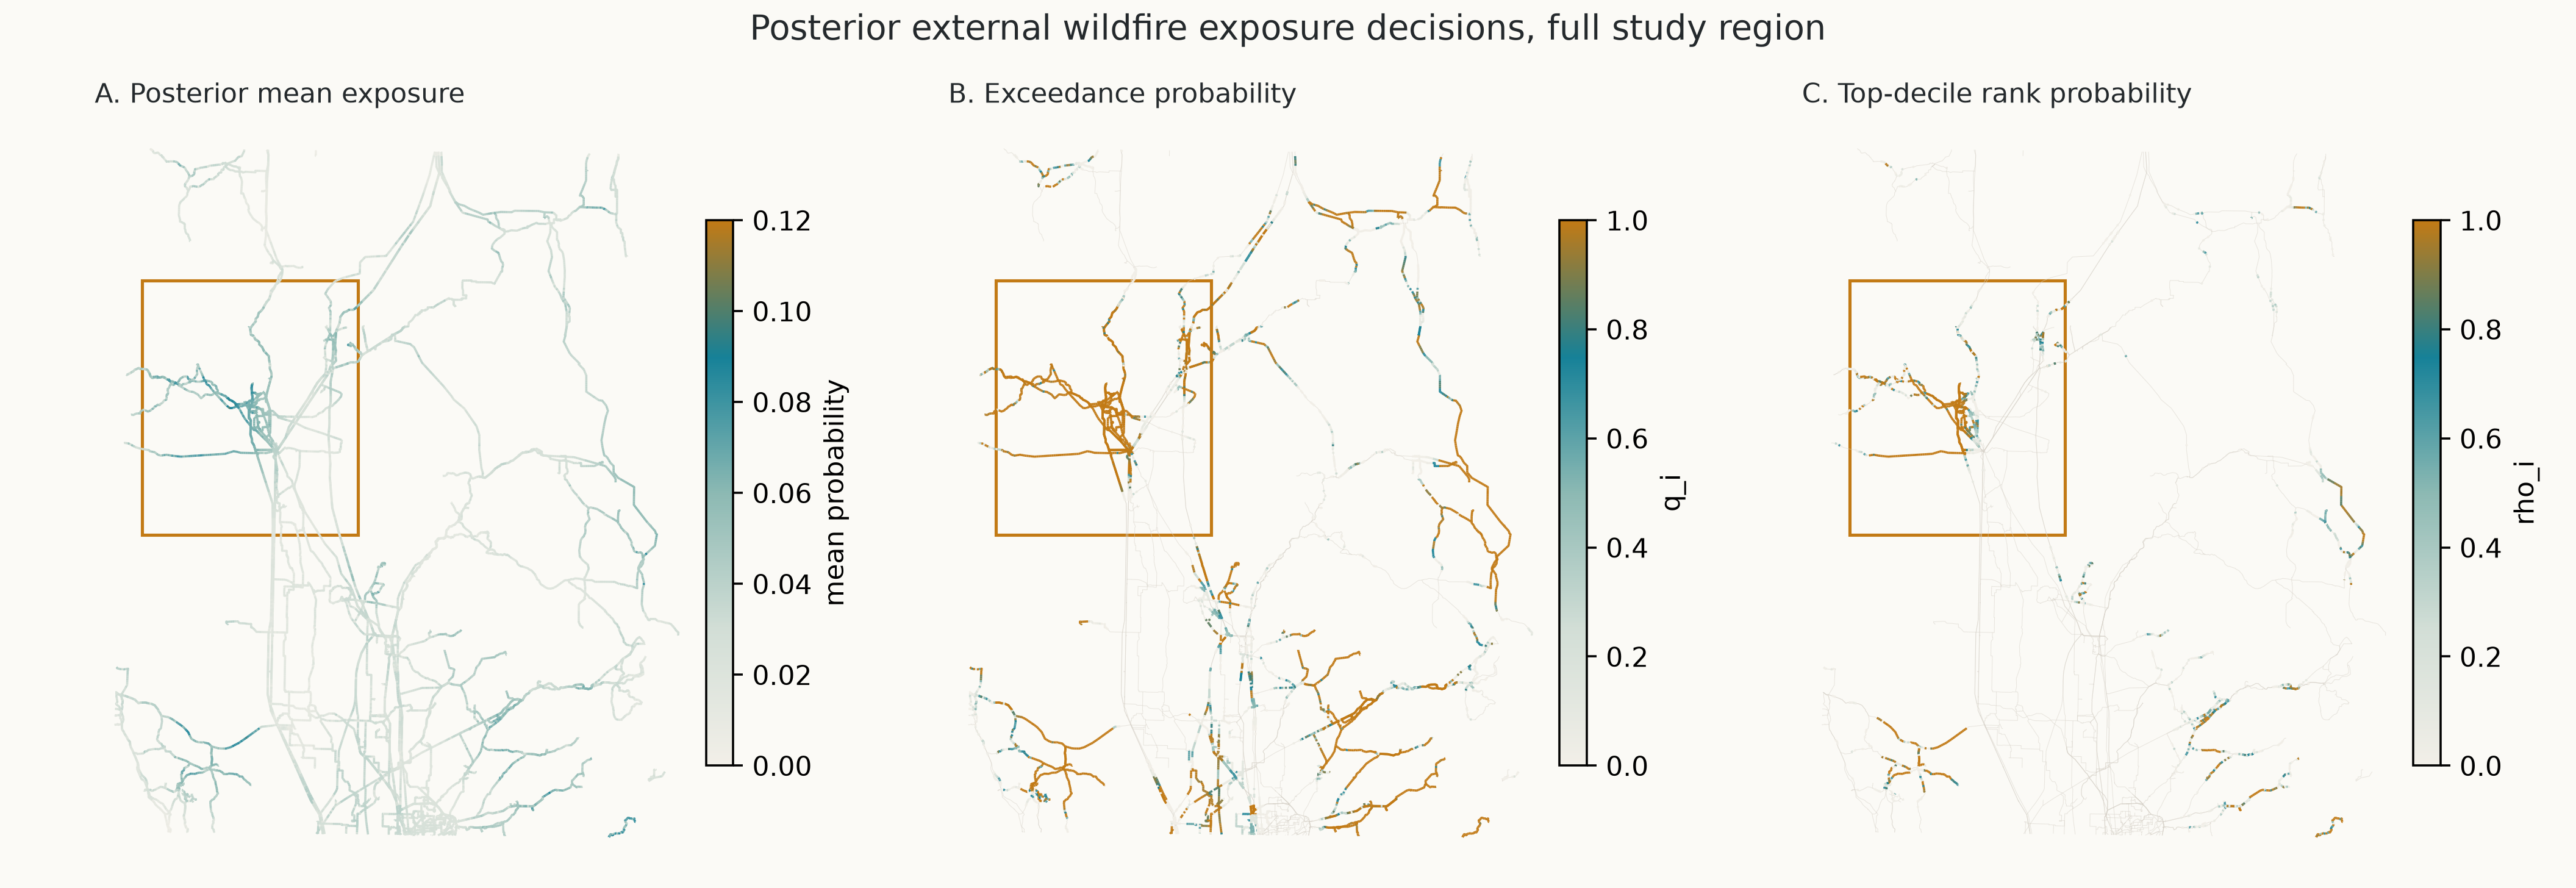
\includegraphics[width=0.96\textwidth]{phase10/phase10_posterior_decision_maps_full_region.png}
  \caption{Full-region maps of posterior mean exposure probability, posterior exceedance probability, and posterior top-decile rank probability.}
  \label{fig:posterior-maps}
\end{figure}

\autoref{tab:rank-uncertainty} summarizes the segment-level decision-set
implication of $\rho_i$. The stable top-decile set contains 781 segments with
$\rho_i\ge0.9$, while 708 segments fall into the rank-uncertain interval
$0.1<\rho_i<0.9$. The point-estimate top decile contains 1,126 segments, but
its Jaccard overlap with the stable posterior top-decile set is 0.694; 27
point-top-decile segments have $\rho_i<0.5$. This shows that a single ranked
list hides decision-relevant rank uncertainty even when point discrimination is
similar to L2 logistic.

\begin{table}[!htbp]
  \centering
  \small
  \caption{Posterior rank uncertainty groups evaluated against 2022--2023 observed segment exposure.}
  \label{tab:rank-uncertainty}
  \begin{tabular}{lrrr}
    \toprule
    Posterior rank group & Segments & Observed exposed segments & Exposure frequency \\
    \midrule
    Stable top-decile ($\rho_i\ge0.9$) & 781 & 41 & 0.0525 \\
    Rank-uncertain ($0.1<\rho_i<0.9$) & 708 & 46 & 0.0650 \\
    Stable lower rank ($\rho_i\le0.1$) & 9,766 & 264 & 0.0270 \\
    \bottomrule
  \end{tabular}
\end{table}

\begin{figure}[!htbp]
  \centering
  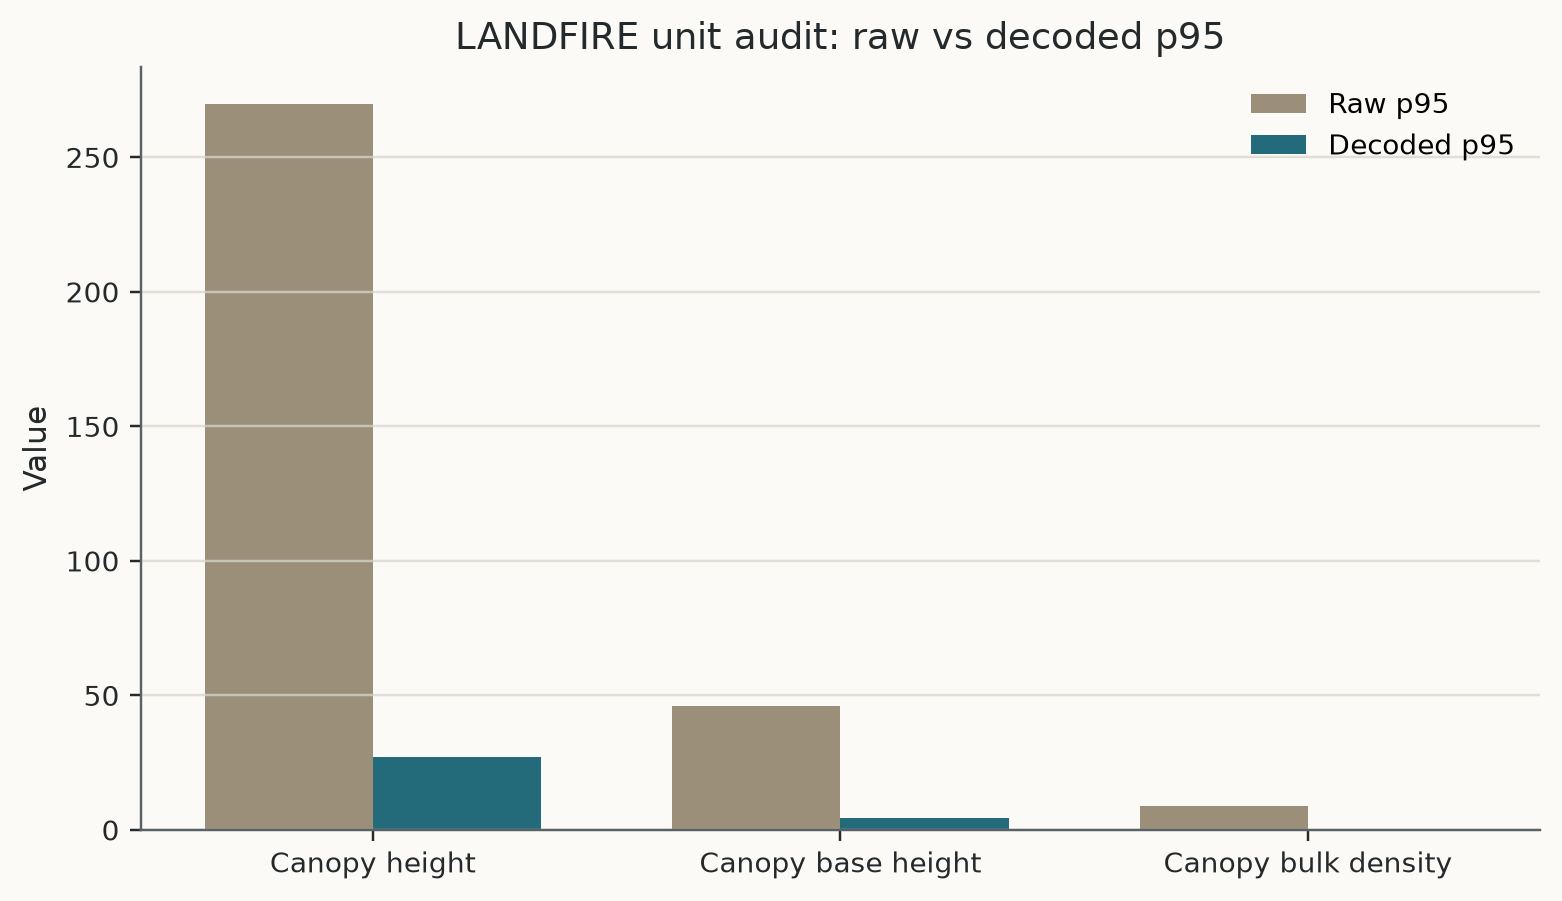
\includegraphics[width=0.80\textwidth]{phase9/phase9_20260707_113214_landfire_scaling_audit.png}
  \caption{LANDFIRE unit audit for canopy height, canopy base height, and canopy bulk density.}
  \label{fig:landfire-audit}
\end{figure}

The selected Bayesian and L2 logistic core does not use FBFM40. The processed
CH, CBH, and CBD columns are positive constant scalings of decoded physical
units; because the selected linear core standardizes these variables before
fitting, decoding does not require rerunning the selected Bayesian/L2 model.
This no-rerun statement does not apply to threshold rules or tree models.
Because feature-core selection was not evaluated with a nested temporal
selection design, the 2022--2023 comparison should be interpreted as a
retrospective model comparison rather than a locked final-test estimate.

\begin{figure}[!htbp]
  \centering
  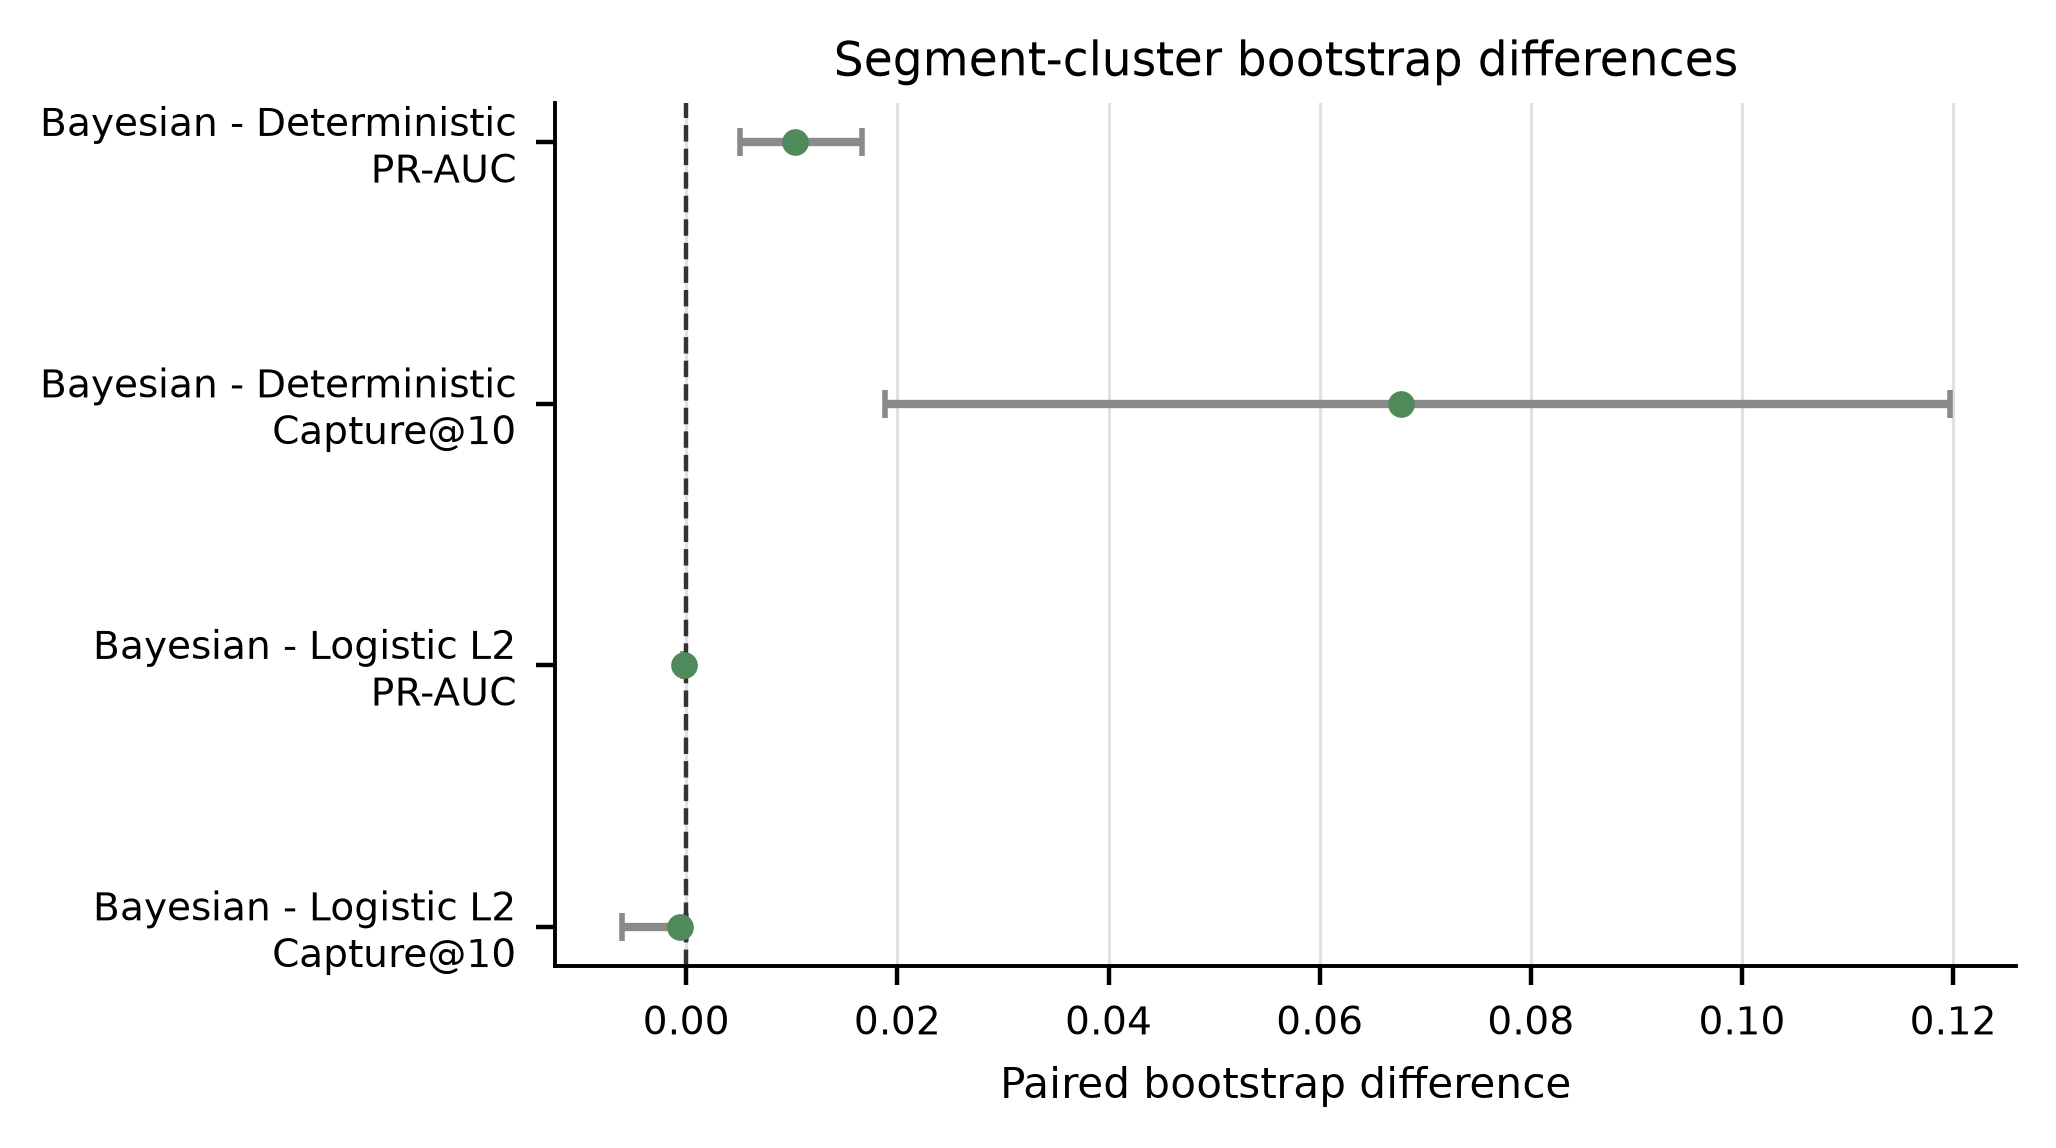
\includegraphics[width=0.78\textwidth]{sci_minorrev_20260708/fig_bootstrap.png}
  \caption{Paired segment-cluster bootstrap differences for PR-AUC and Capture@10. Bayesian Laplace improves Capture@10 relative to the deterministic comparator in this split, while Bayesian Laplace and L2 logistic are nearly indistinguishable by this check.}
  \label{fig:bootstrap}
\end{figure}
\FloatBarrier

\section{Discussion}

The main result is bounded. Public data can support a reproducible,
screening-level framework for retrospective external wildfire exposure ranking
of transmission-line receptor assets. The output is a ranked exposure screen,
not a statement about ignition causality, equipment condition, outage, damage,
or responsibility.

The temporal-holdout results do not show broad Bayesian classification
superiority. L2 logistic and Bayesian Laplace have nearly identical ROC-AUC,
PR-AUC, Brier score, and top-decile capture. This is consistent with the
relationship between Gaussian-prior logistic regression and L2 penalization.
The Bayesian contribution is instead decision-facing: posterior draws convert a
fitted exposure model into posterior exceedance probability and posterior
top-decile rank probability.

The deterministic comparator remains useful because it is transparent and easy
to audit. Its limitation is that it gives one ranking without posterior rank
uncertainty. Flexible tree-based ML baselines do not improve this temporal
holdout, but this result should be interpreted cautiously. It supports careful
feature design and temporal validation, not a general rejection of ML.

Existing wildfire risk tools target different questions. Powerline ignition
models generally require private utility data and address grid-to-fire
causality \citep{yao2022electricityWildfire}. Fire-to-grid and grid-impact
studies address consequences for electricity systems
\citep{dale2018californiaGrid,panossianElgindy2023wildfire}. Physical and
quasi-physical fire-spread models target propagation dynamics and require a
different set of process and scenario assumptions \citep{sullivan2009spread}.
The present framework occupies a narrower space: public-data fire-to-grid
external exposure ranking with a posterior decision layer.

\section{Limitations}

Several limitations are important. First, the pipeline estimates external
exposure only. It does not estimate ignition causality, equipment failure,
outage probability, damage, or legal responsibility. Second, the CAL FIRE cause
field is a perimeter-level attribute; electrical-power overlap is therefore
only a diagnostic label. Third, LF2024 static fuel layers may be temporally
mismatched with 2017--2023 exposure years \citep{landfire2024update}. Fourth,
FBFM40 must be encoded categorically or removed from final ablations. Fifth,
the label uses a fixed 1 km buffer, so buffer-radius sensitivity remains a
model-definition sensitivity. Sixth, temporal holdout does not remove spatial
dependence among neighboring segments. Blocked validation is recommended when
spatial or hierarchical dependence structures are present
\citep{roberts2017crossvalidation}; spatially separated folds can be
operationalized with block-based procedures \citep{valavi2019blockcv}. Finally,
the Stan run is a pilot; full diagnostics, longer chains, convergence
summaries, and posterior predictive checks remain necessary for stronger
Bayesian computation claims.

\section{Conclusion}

This paper presents a public-data framework for retrospective external wildfire
exposure ranking of transmission-line receptor assets. The workflow builds a
2017--2023 segment-year panel, uses cause-screened exposure labels, and compares
deterministic, Bayesian, and machine-learning baselines under a 2022--2023
temporal holdout. Bayesian and L2 logistic point-prediction performance is
similar. The Bayesian formulation adds posterior exceedance and posterior
top-decile rank probabilities, with posterior rank probability emphasized as
the main decision quantity. The framework should not be interpreted as a
powerline ignition, equipment-failure, outage, damage, or responsibility model.

\appendix

\section{Posterior Map Zoom}

\begin{figure}[!htbp]
  \centering
  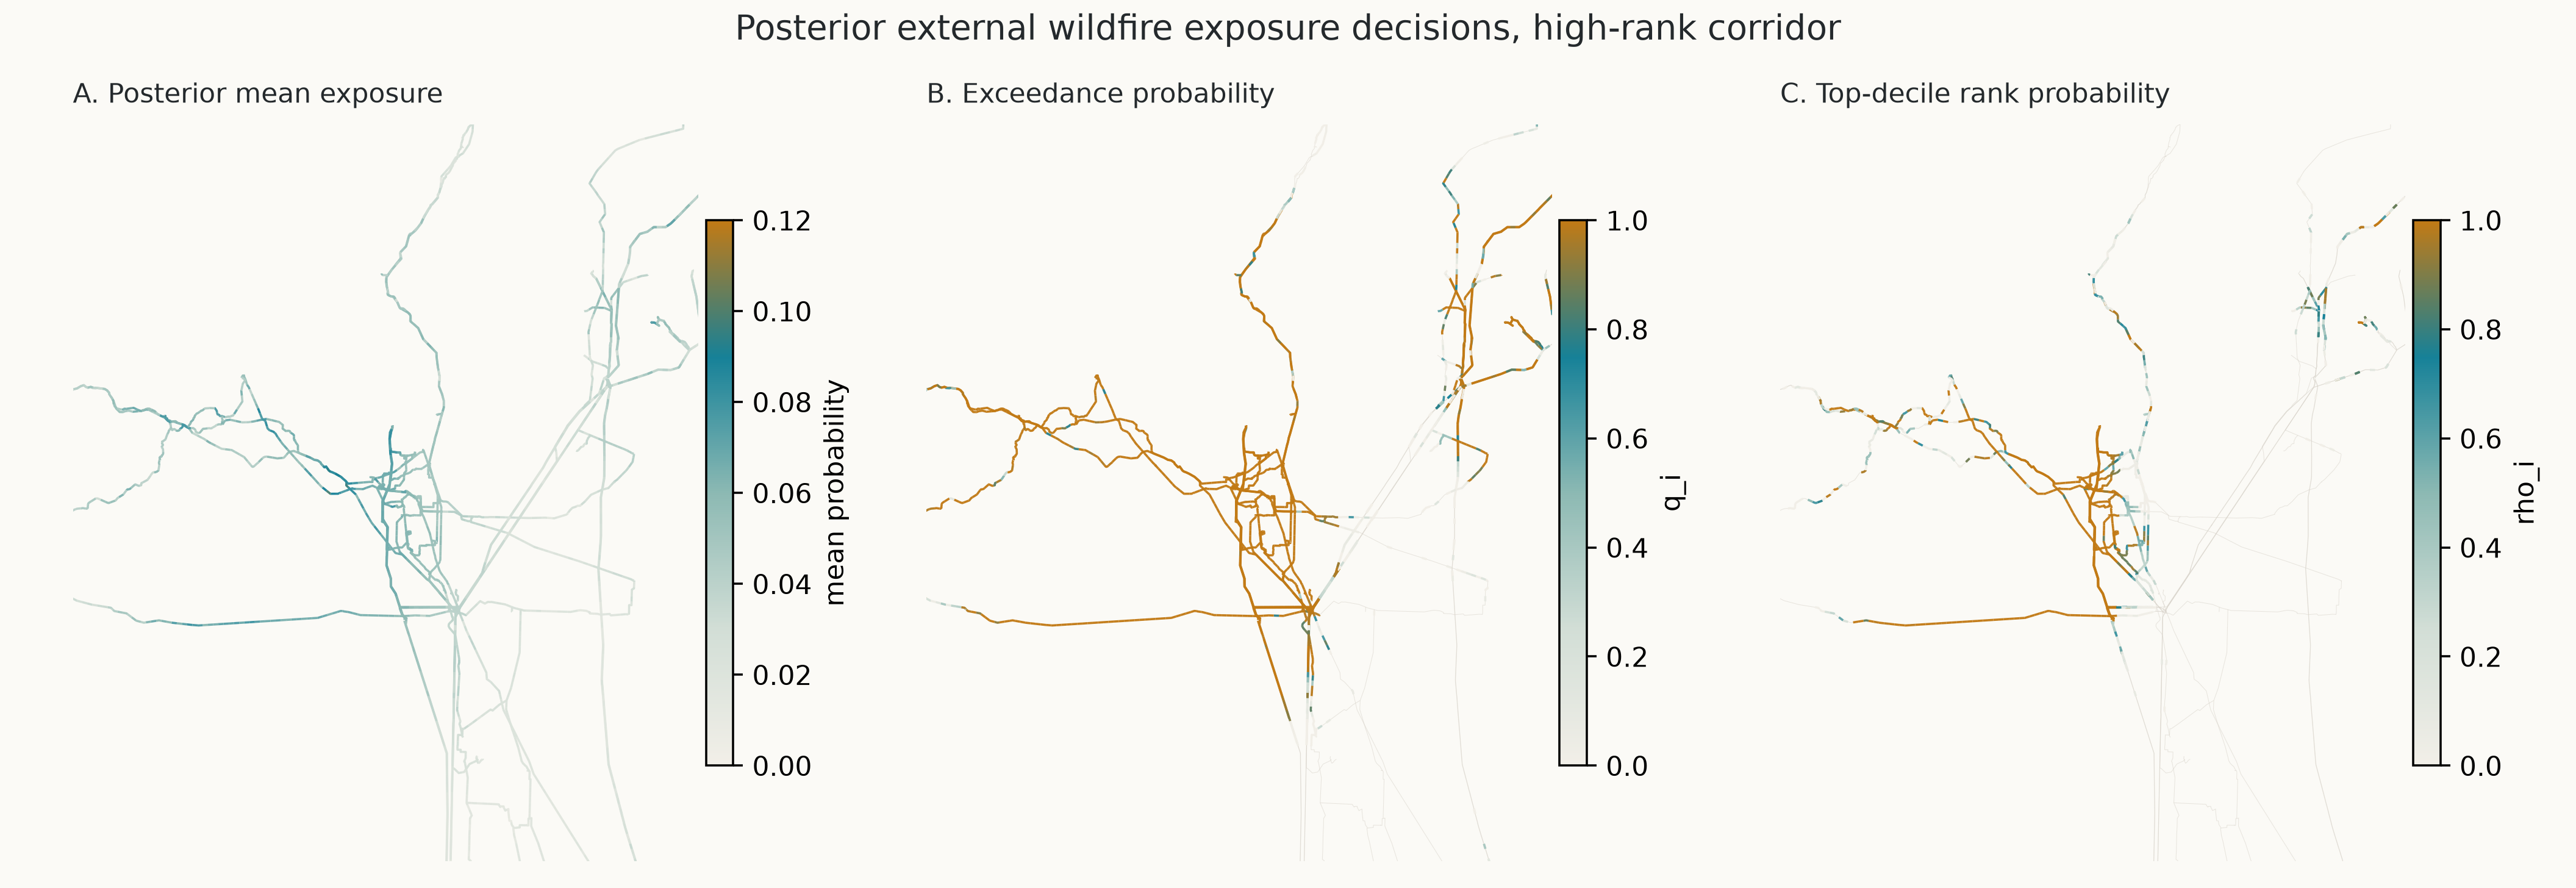
\includegraphics[width=0.96\textwidth]{phase10/phase10_posterior_decision_maps_zoom_corridor.png}
  \caption{Zoomed high-rank corridor for posterior mean exposure probability, posterior exceedance probability, and posterior top-decile rank probability.}
  \label{fig:posterior-maps-zoom}
\end{figure}

\section{Covariate Diagnostics}

The following maps document the public covariate layers used to construct
dynamic weather, terrain, and fuel-structure predictors. They are included as
covariate-diagnostic figures rather than as separate scientific claims.

\begin{figure}[!htbp]
  \centering
  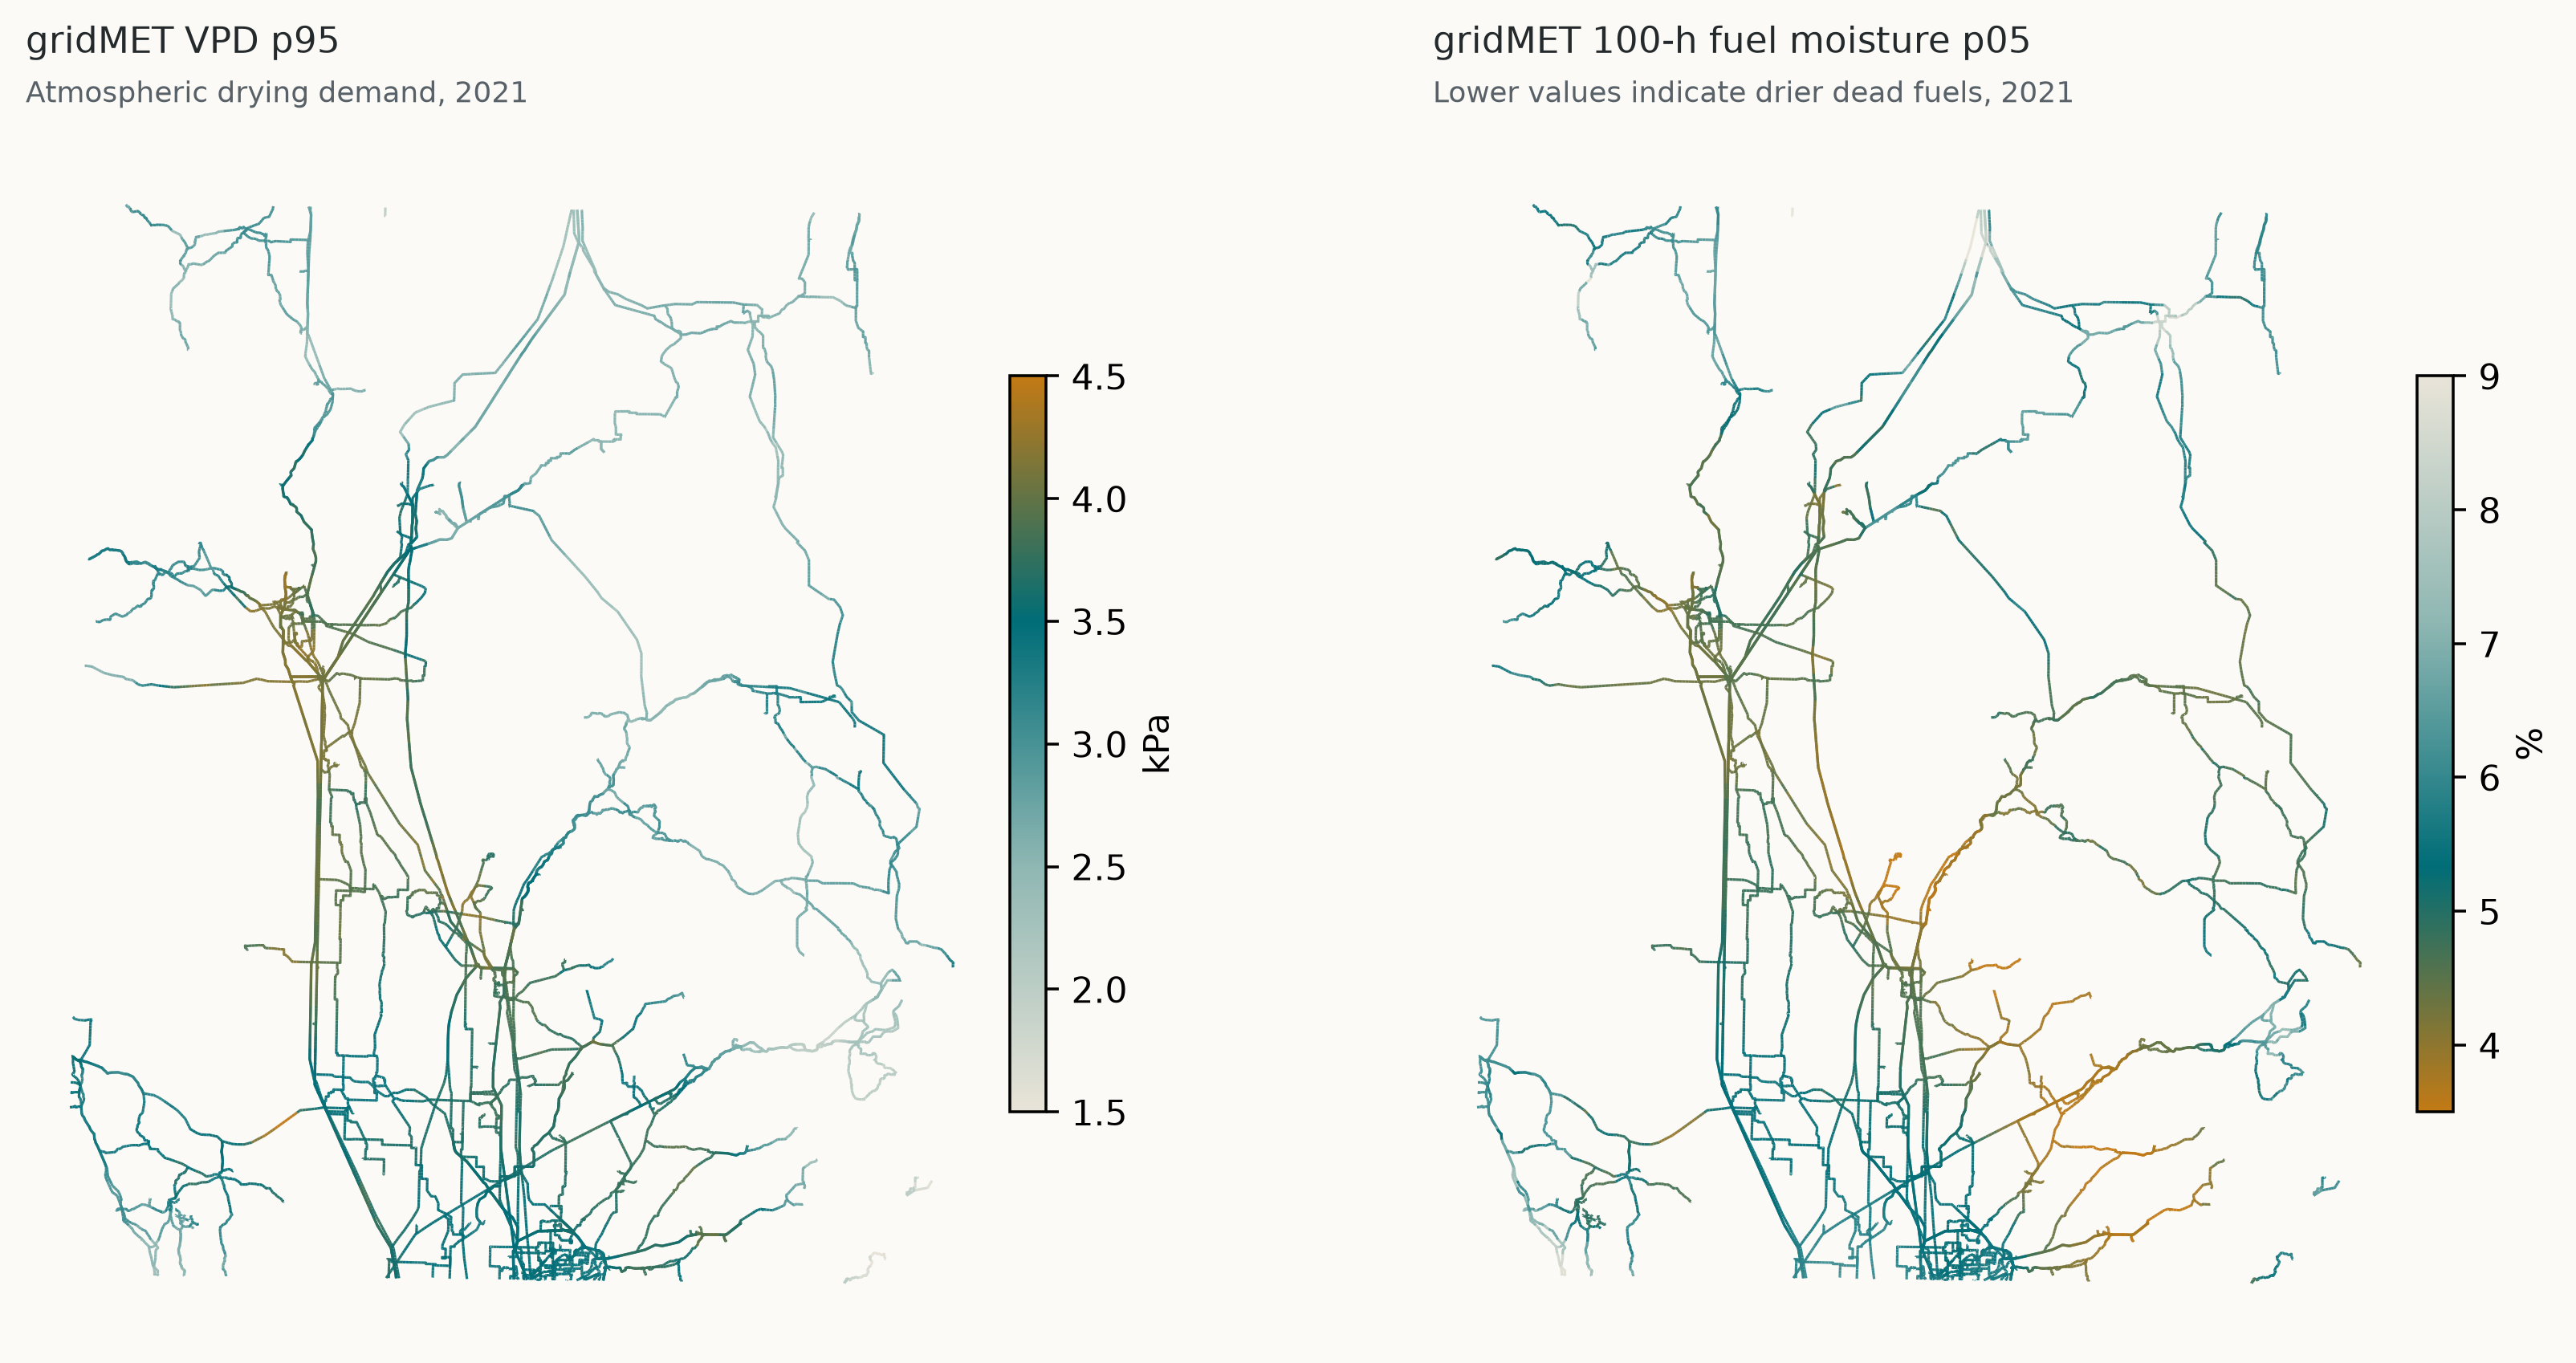
\includegraphics[width=0.92\textwidth]{phase8/phase8_gridmet_model_covariates_2021.png}
  \caption{gridMET annual fire-weather covariate layers for 2021.}
  \label{fig:gridmet-layers}
\end{figure}

\begin{figure}[!htbp]
  \centering
  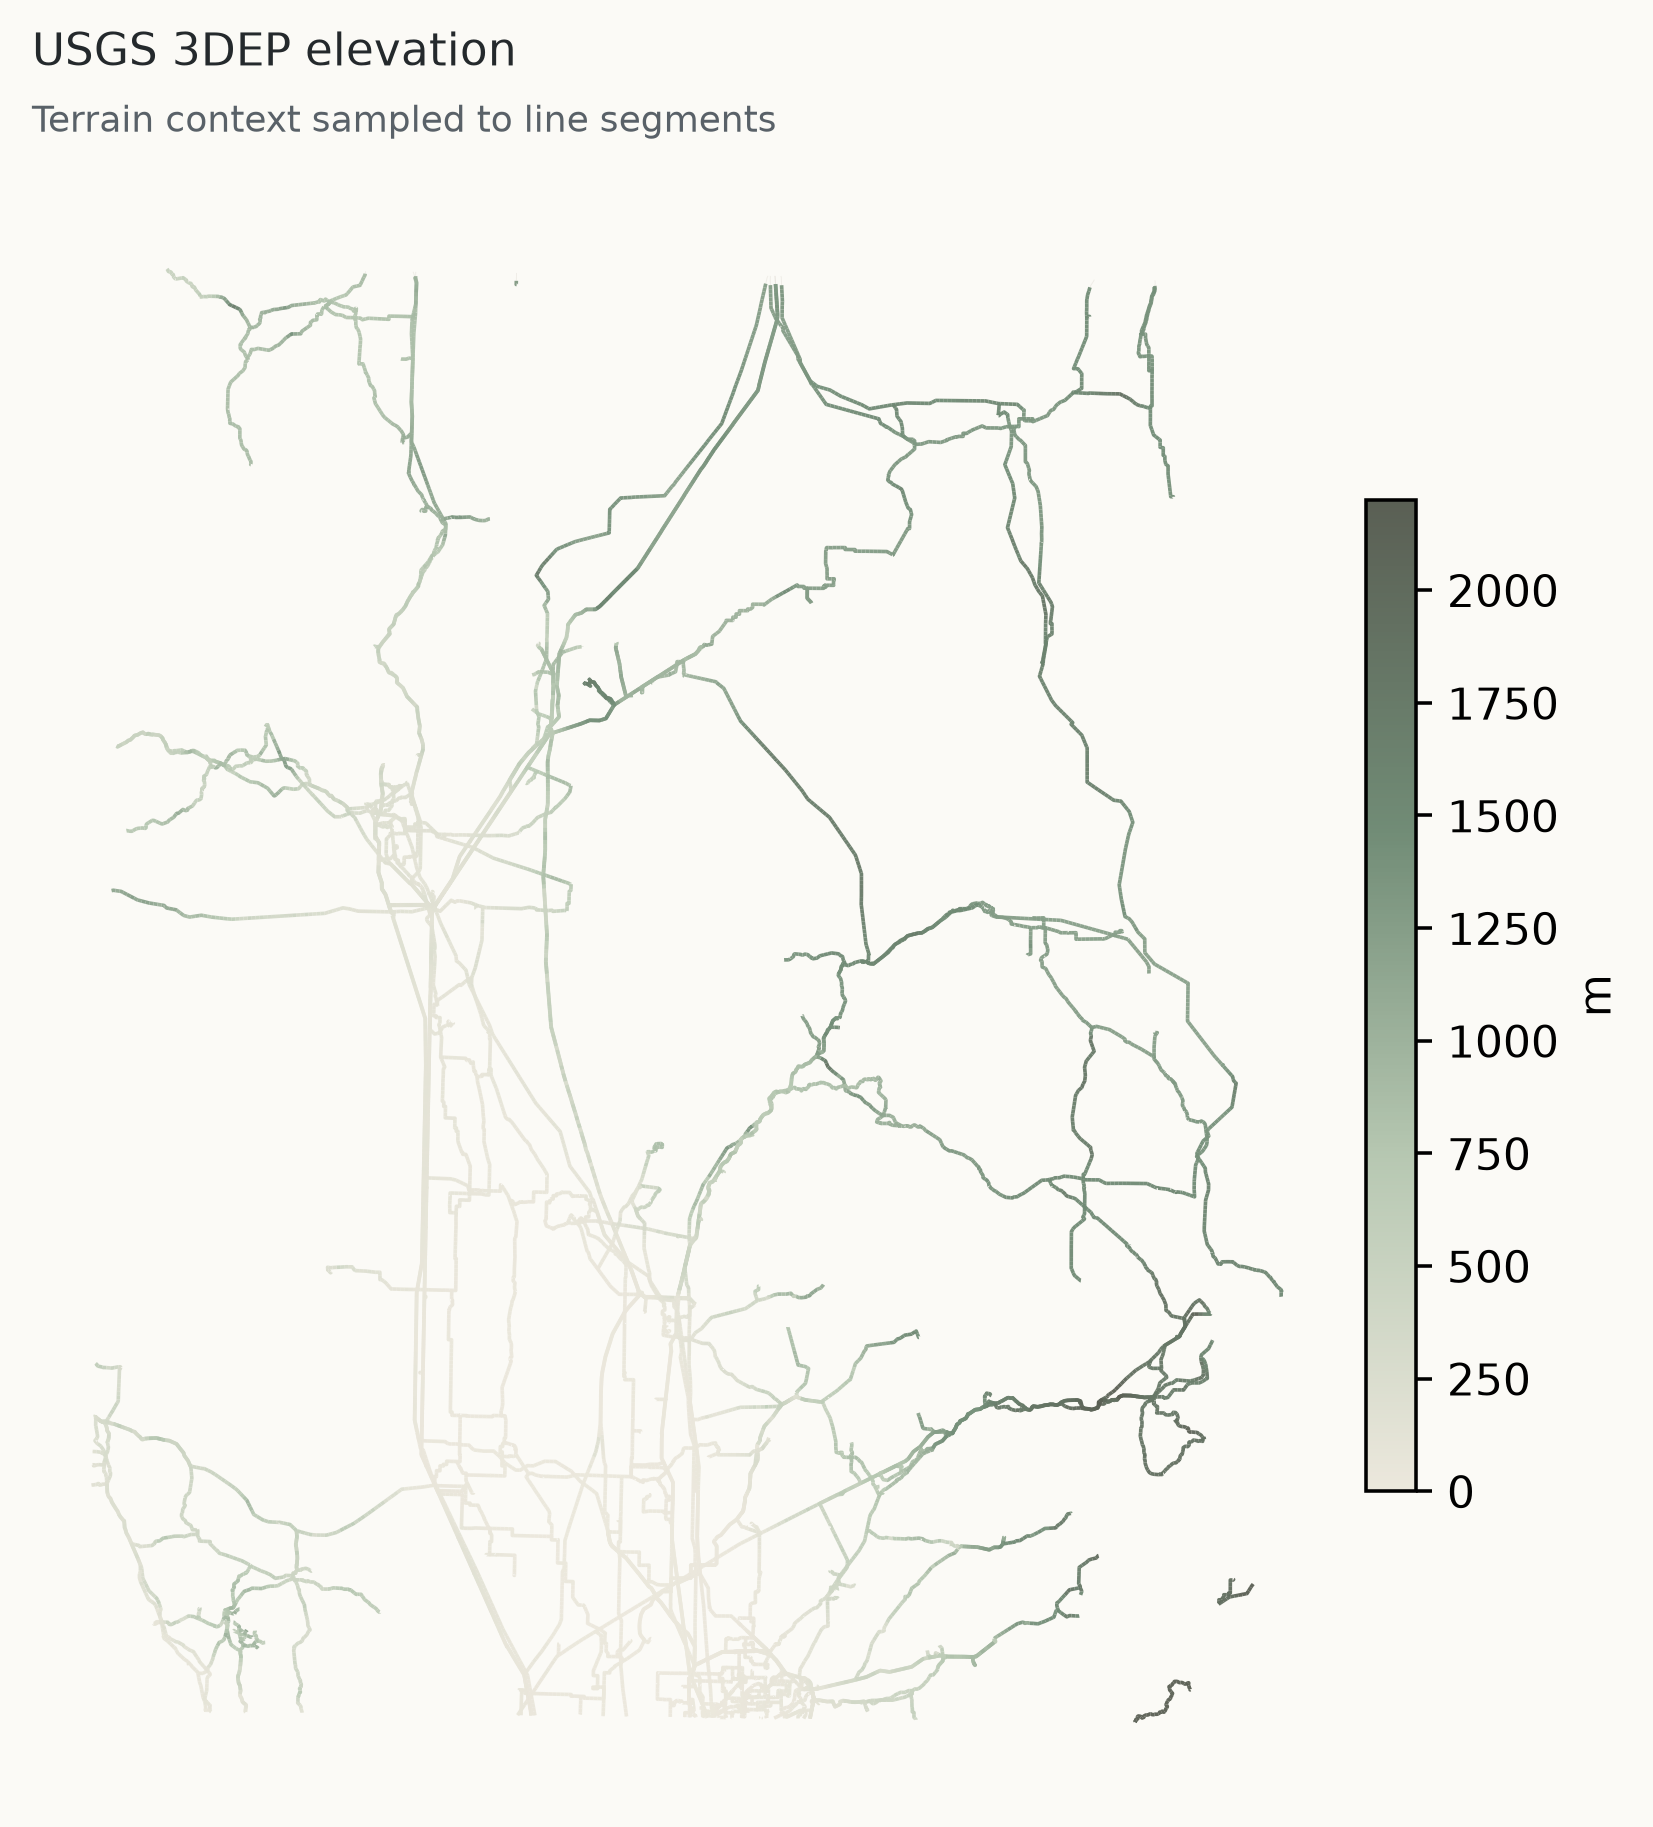
\includegraphics[width=0.86\textwidth]{phase8/phase8_dem_model_covariate.png}
  \caption{USGS 3DEP terrain covariate layer.}
  \label{fig:dem-layers}
\end{figure}

\begin{figure}[!htbp]
  \centering
  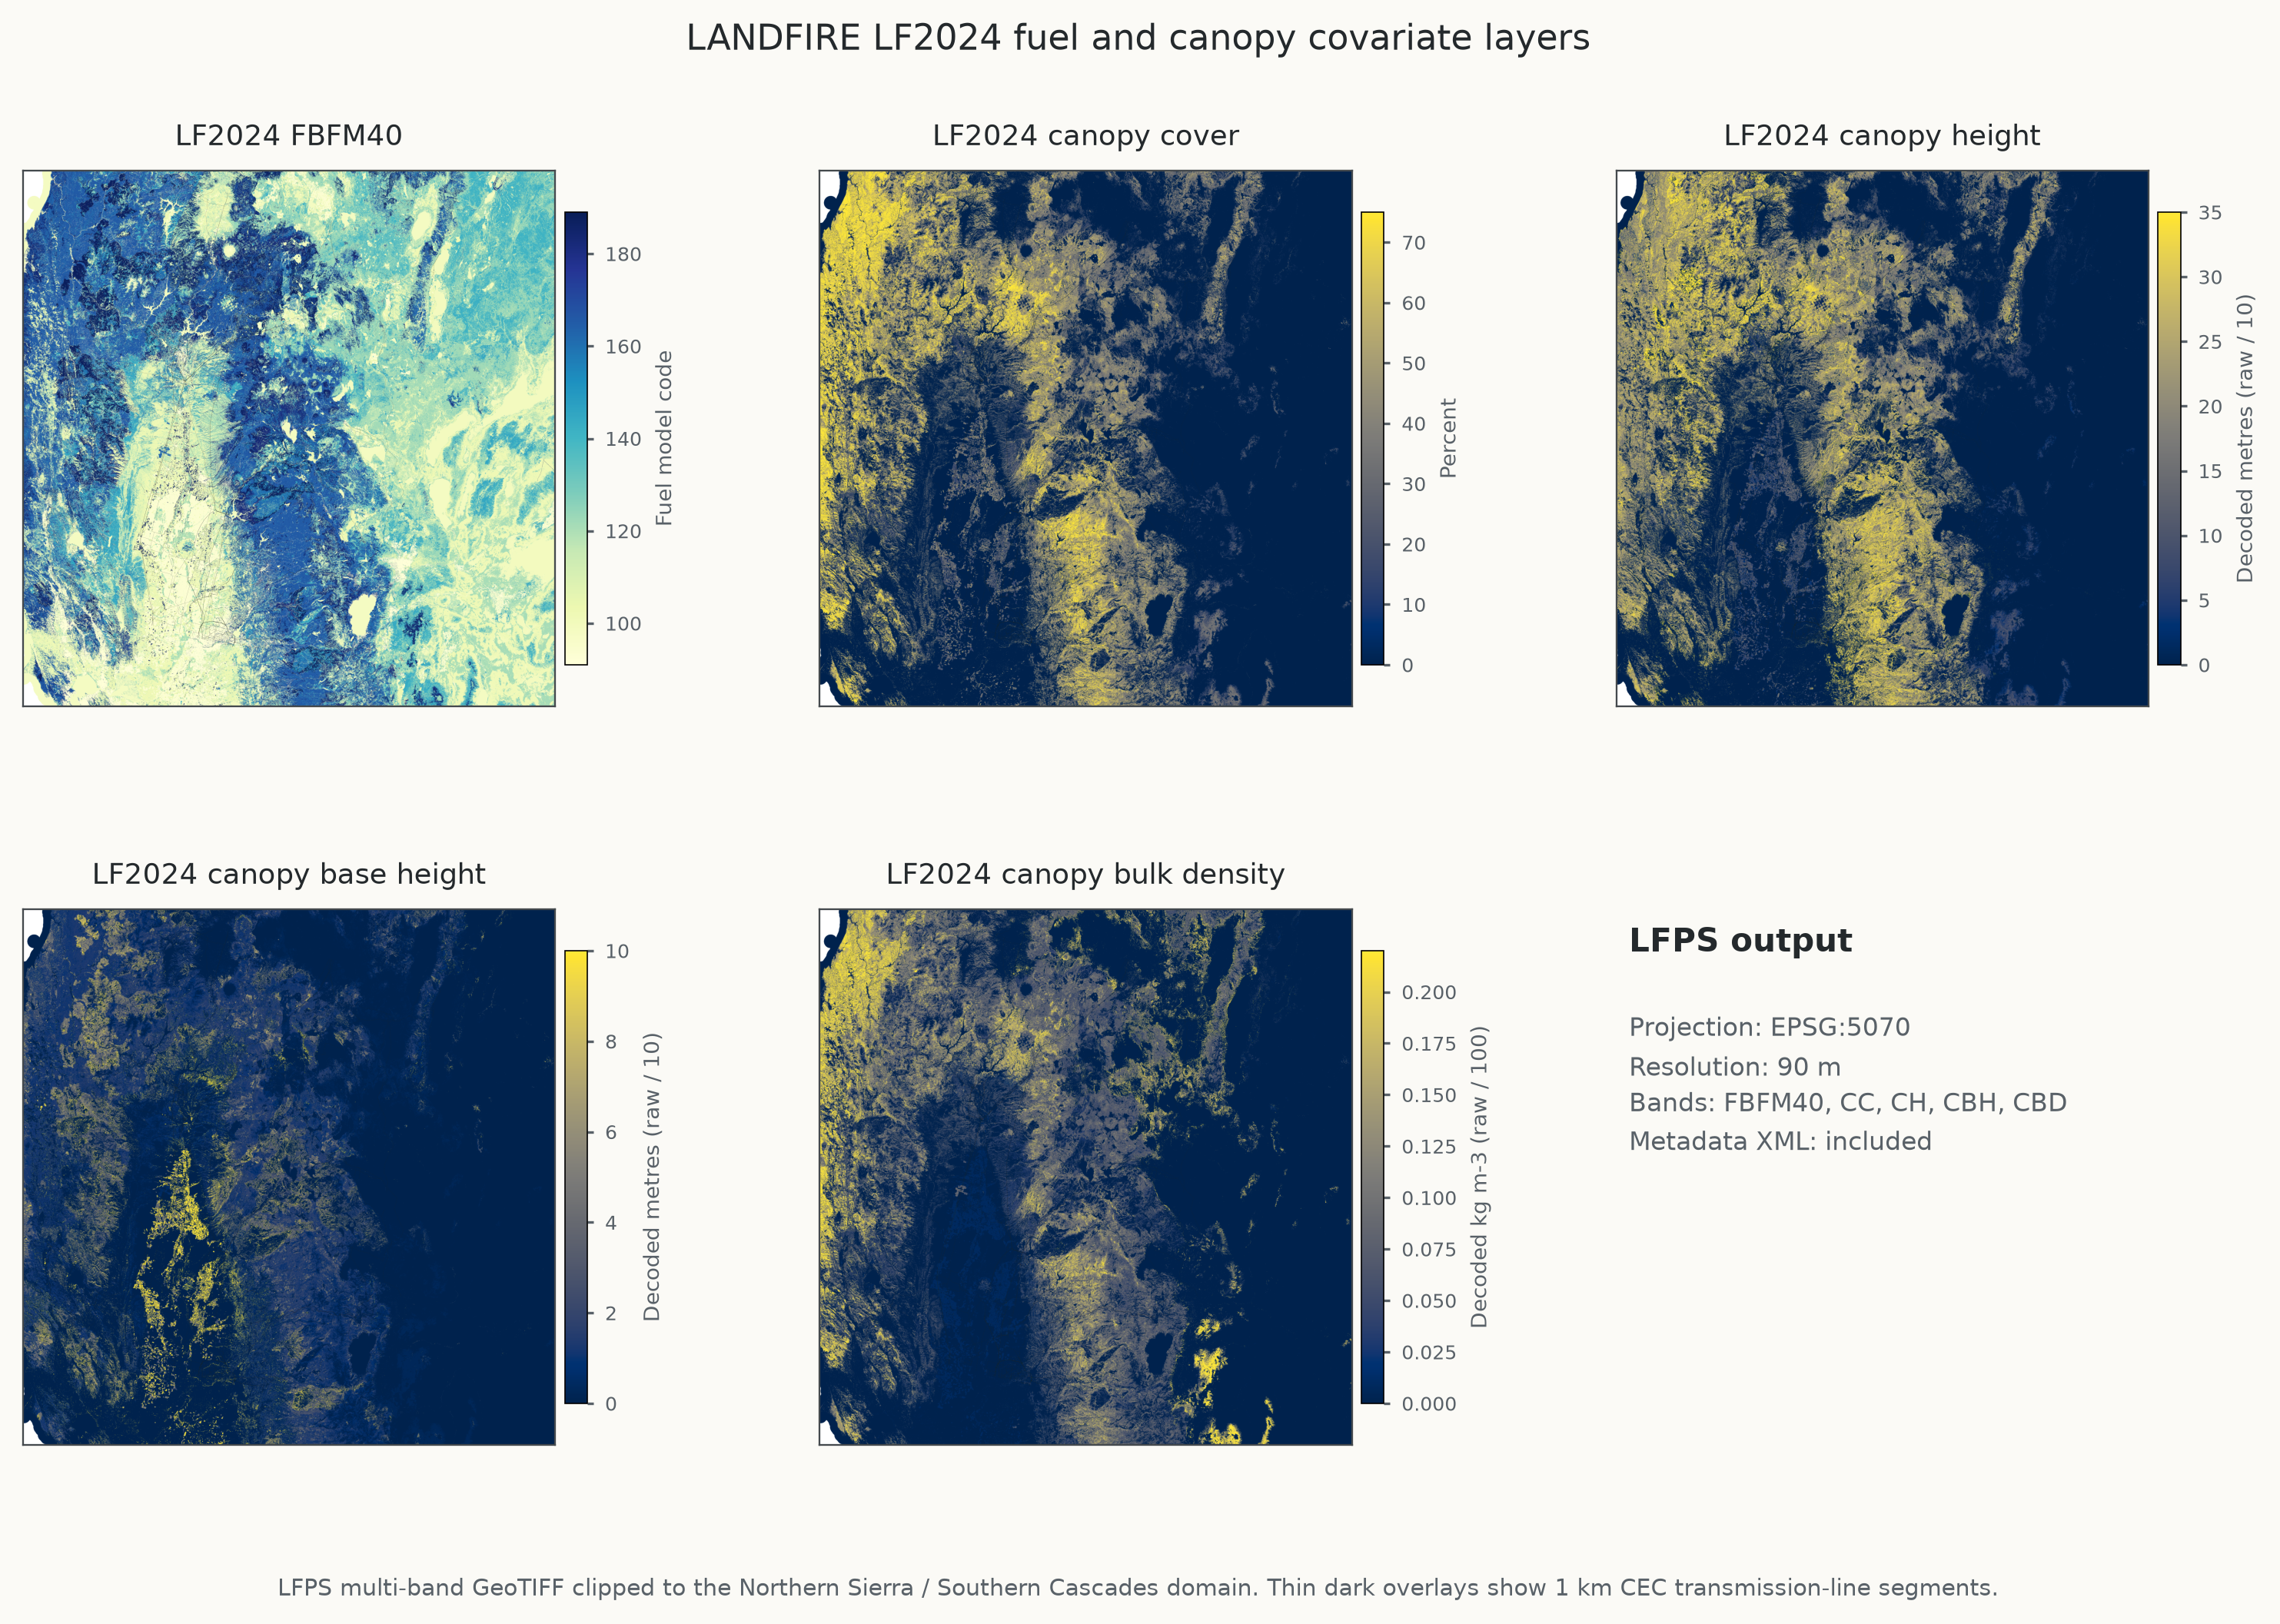
\includegraphics[width=0.92\textwidth]{data_previews/phase2_landfire_covariate_layers.png}
  \caption{LANDFIRE LF2024 fuel and canopy covariate layers with decoded CH, CBH, and CBD units.}
  \label{fig:landfire-layers}
\end{figure}

\begin{figure}[!htbp]
  \centering
  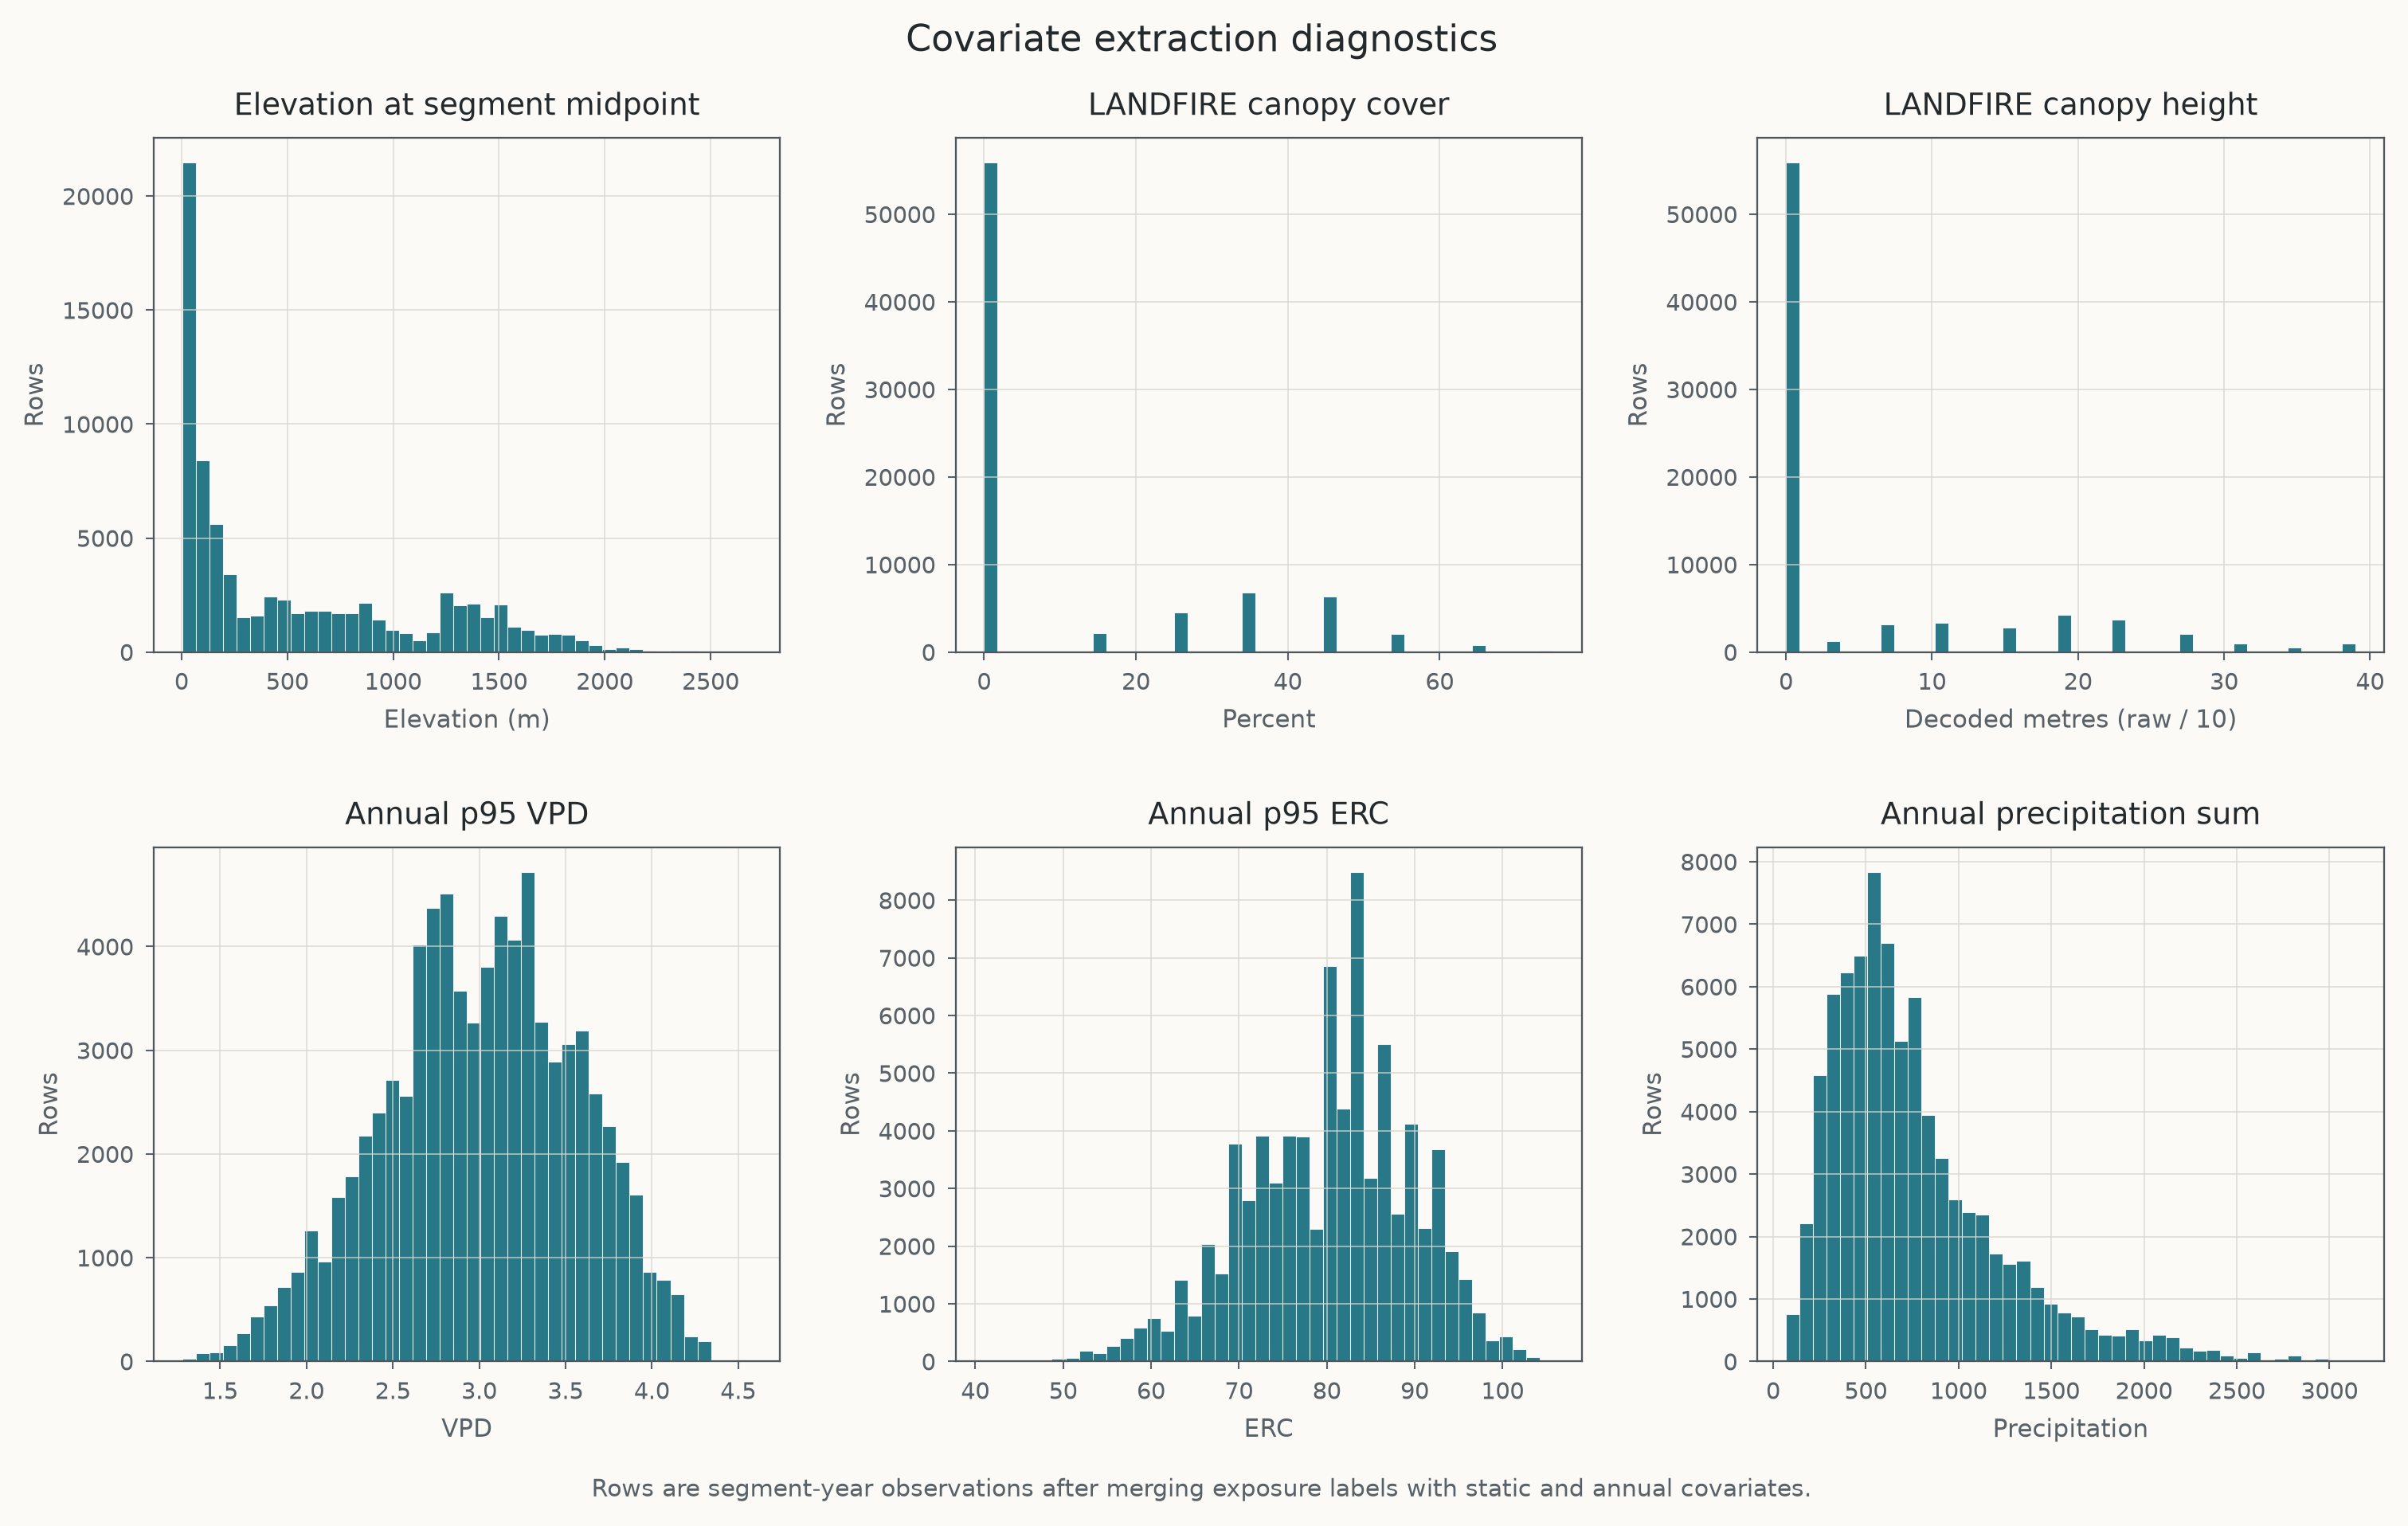
\includegraphics[width=0.92\textwidth]{phase3/phase3_covariate_qc_distributions.png}
  \caption{Covariate distribution diagnostics with decoded LANDFIRE canopy height units.}
  \label{fig:covariate-distributions}
\end{figure}

\begin{figure}[!htbp]
  \centering
  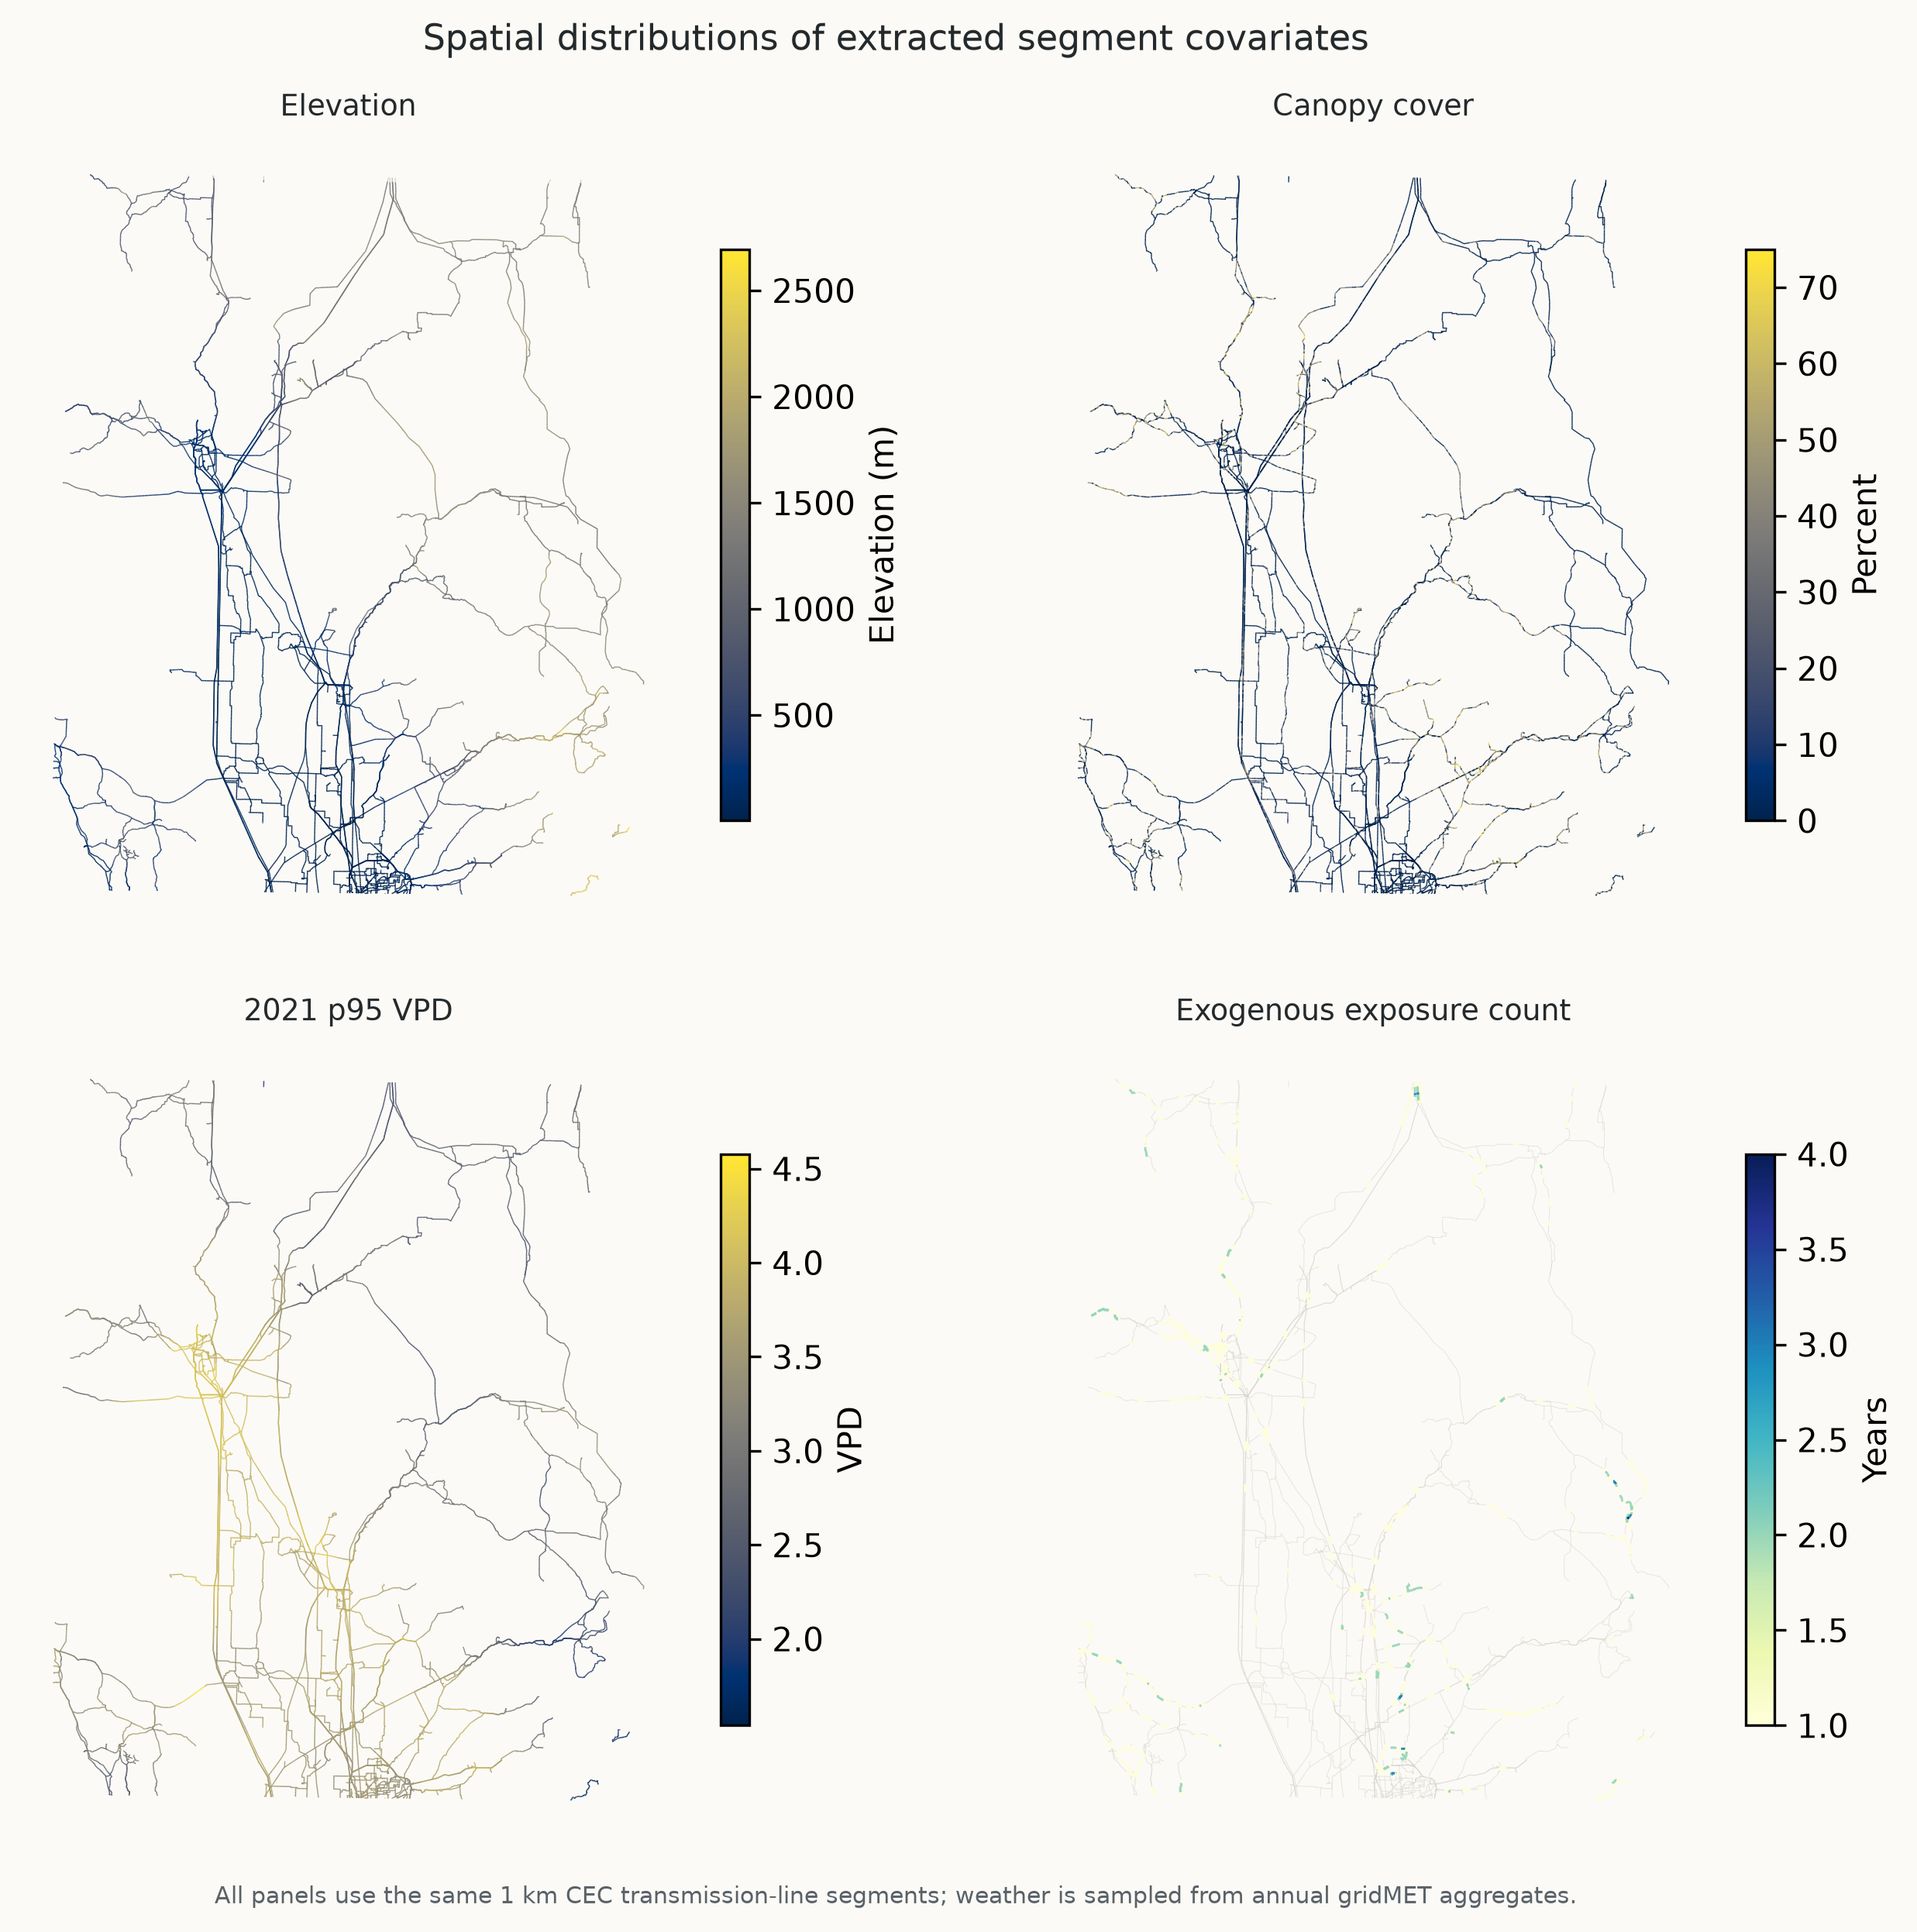
\includegraphics[width=0.92\textwidth]{phase3/phase3_spatial_qc_maps.png}
  \caption{Spatial covariate distributions.}
  \label{fig:spatial-qc}
\end{figure}

\FloatBarrier
\clearpage

\bibliographystyle{plainnat}
\bibliography{references_wildfire_exposure_verified}

\end{document}
